\documentclass[12pt, letterpaper]{article}

% ============================================================
% PAQUETES
% ============================================================

\usepackage[utf8]{inputenc}
\usepackage[T1]{fontenc}
\usepackage[spanish, es-tabla]{babel}
\usepackage{lmodern}
\usepackage{geometry}
\usepackage{setspace}
\usepackage{amsmath, amssymb}
\usepackage{graphicx}
\usepackage{tikz}
\usetikzlibrary{shapes.geometric, arrows.meta, positioning, calc}
\usepackage{float}
\usepackage{booktabs}
\usepackage{array}
\usepackage{tabularx}
\usepackage{longtable}
\usepackage{hyperref}
\usepackage{caption}
\usepackage{subcaption}
\usepackage{siunitx}
\usepackage{enumitem}
\usepackage{xurl}
\usepackage{microtype}
\usepackage{fancyhdr}
\usepackage{xcolor}

% ============================================================
% CONFIGURACION GENERAL
% ============================================================

\geometry{
    left=2.2cm,
    right=2.2cm,
    top=2.2cm,
    bottom=2.2cm,
    headheight=20pt,
    headsep=0.5cm
}
\setlength{\floatsep}{8pt plus 2pt minus 2pt}
\setlength{\textfloatsep}{10pt plus 2pt minus 2pt}
\setlength{\intextsep}{8pt plus 2pt minus 2pt}

\AtBeginDocument{\fontsize{12pt}{15.5pt}\selectfont}
\setstretch{1.30}
\setlength{\parindent}{0pt}
\setlength{\parskip}{0.40em}
\renewcommand{\arraystretch}{1.18}

\hypersetup{
    colorlinks=true,
    linkcolor=black,
    citecolor=black,
    urlcolor=blue
}

\sisetup{
    output-decimal-marker = {,},
    per-mode = symbol
}

\graphicspath{{outputs/03_diagnostico_fd_santiago/}{outputs/04_modelo_hibrido_xgboost_santiago/}}

\fancypagestyle{informe}{
    \fancyhf{}
    \fancyhead[L]{%
        \IfFileExists{uandresbello.png}{%
            \raisebox{0.08cm}{
\includegraphics[height=0.47cm]{uandresbello.png}}%
        }{}%
    }
    \fancyhead[R]{\thepage}
    \renewcommand{\headrulewidth}{0.4pt}
    \renewcommand{\footrulewidth}{0pt}
}
\fancypagestyle{plain}{%
    \fancyhf{}
    \fancyhead[L]{%
        \IfFileExists{uandresbello.png}{%
            \raisebox{0.08cm}{
\includegraphics[height=0.47cm]{uandresbello.png}}%
        }{}%
    }
    \fancyhead[R]{\thepage}
    \renewcommand{\headrulewidth}{0.4pt}
    \renewcommand{\footrulewidth}{0pt}
}

% ============================================================
% DATOS DEL DOCUMENTO
% ============================================================

\newcommand{\universidad}{Universidad Andr\'es Bello}
\newcommand{\facultad}{Facultad de Ciencias Exactas}
\newcommand{\carrera}{Ingenier\'ia F\'isica}
\newcommand{\tituloTesis}{Evaluaci\'on de un modelo h\'ibrido f\'isico--informado para la estimaci\'on de potencia fotovoltaica bajo distintos reg\'imenes de fracci\'on difusa}
\newcommand{\autor}{Nicol\'as Antonio Aravena Osorio}
\newcommand{\profesor}{Eduardo Jeraldo}
\newcommand{\ciudad}{Santiago, Chile}
\newcommand{\fecha}{Julio, 2026}

% ============================================================
% DOCUMENTO
% ============================================================

\begin{document}
\hypersetup{pageanchor=false}

% ============================================================
% PORTADA
% ============================================================

\begin{titlepage}
    \thispagestyle{empty}
    \begingroup
    \centering
    \setstretch{1.0}
    \setlength{\parskip}{0pt}
    \fontsize{12pt}{14pt}\selectfont

    \vspace*{-0.55cm}

    \IfFileExists{uandresbello.png}{%
        
\includegraphics[height=2.55cm]{uandresbello.png}\par
    }{%
        \vspace*{2.55cm}
    }

    \vspace{0.75cm}

    {\fontsize{17.5pt}{19pt}\selectfont
    UNIVERSIDAD ANDR\'ES BELLO\par
    FACULTAD DE CIENCIAS\par
    EXACTAS\par}

    \vspace{1.05cm}

    {\fontsize{12.5pt}{15pt}\selectfont Proyecto de T\'itulo Ingenier\'ia F\'isica\par}

    \vspace{1.05cm}

    {\fontsize{14.2pt}{16.2pt}\selectfont
    \begin{minipage}{0.78\textwidth}
    \centering
    Evaluaci\'on de un Modelo H\'ibrido F\'isico--Informado para la Estimaci\'on de Potencia Fotovoltaica bajo Distintos Reg\'imenes de Fracci\'on Difusa
    \end{minipage}\par}

    \vspace{1.35cm}

    {\fontsize{11.5pt}{14pt}\selectfont\textbf{Autor:}\par}
    \vspace{0.18cm}
    {\fontsize{10.5pt}{13pt}\selectfont\textit{\autor}\par}

    \vspace{0.72cm}

    {\fontsize{11.5pt}{14pt}\selectfont\textbf{Profesor Gu\'ia:}\par}
    \vspace{0.18cm}
    {\fontsize{10.5pt}{13pt}\selectfont\textit{\profesor}\par}

    \vspace{4.25cm}

    {\fontsize{10.5pt}{13pt}\selectfont \fecha\par}
    \vspace{0.18cm}
    {\fontsize{10.5pt}{13pt}\selectfont \ciudad\par}
    \endgroup

\end{titlepage}

\hypersetup{pageanchor=true}
\pagenumbering{arabic}
\pagestyle{informe}

% ============================================================
% INDICE
% ============================================================

\tableofcontents
\newpage
\listoffigures
\newpage
\listoftables
\newpage
\section*{Nomenclatura}
\addcontentsline{toc}{section}{Nomenclatura}
\begin{itemize}[label={}]
    \item \textbf{$P_{ref}$}: Potencia DC simulada de referencia.
    \item \textbf{$\epsilon$}: Residuo o error del modelo f\'isico.
    \item \textbf{$fd$}: Fracci\'on difusa ($DHI / GHI$).
    \item \textbf{$\gamma$}: Coeficiente t\'ermico del m\'odulo fotovoltaico.
    \item \textbf{$\theta_z$}: \'Angulo cenital solar.
    \item \textbf{$GHI$}: Irradiancia global horizontal.
    \item \textbf{$DHI$}: Irradiancia difusa horizontal.
    \item \textbf{$DNI$}: Irradiancia directa normal.
    \item \textbf{$POA$}: Irradiancia sobre el plano del arreglo.
    \item \textbf{NOCT}: Nominal Operating Cell Temperature.
\end{itemize}
\newpage

% ============================================================
% RESUMEN
% ============================================================

\section*{Resumen}
\addcontentsline{toc}{section}{Resumen}

La estimaci\'on de potencia fotovoltaica depende de la correcta representaci\'on de la irradiancia incidente sobre el arreglo fotovoltaico y de las condiciones ambientales que afectan la temperatura de operaci\'on de las celdas. Los modelos f\'isicos simplificados, como el modelo basado en NOCT (\textit{Nominal Operating Cell Temperature}), permiten estimar potencia a partir de variables f\'isicas principales, tales como la irradiancia sobre el plano del panel y la temperatura ambiente. Sin embargo, estos modelos no representan de manera expl\'icita la composici\'on directa y difusa de la radiaci\'on solar, lo que puede introducir diferencias respecto a modelos de referencia m\'as completos.

En este trabajo se eval\'ua un modelo h\'ibrido f\'isico--informado para estimar potencia fotovoltaica. El modelo f\'isico base corresponde a NOCT, mientras que la correcci\'on del residuo del modelo f\'isico se formula mediante aprendizaje residual con XGBoost. La variable central del an\'alisis es la fracci\'on difusa, definida como
\[
    fd = \frac{DHI}{GHI},
\]
donde \(DHI\) corresponde a la irradiancia difusa horizontal y \(GHI\) a la irradiancia global horizontal. Esta variable permite clasificar las condiciones de irradiancia en tres reg\'imenes: baja fracci\'on difusa, r\'egimen mixto y alta fracci\'on difusa.

La metodolog\'ia se implement\'o en cuatro componentes computacionales: descarga y preparaci\'on de datos horarios desde PVWatts para Santiago, c\'alculo del modelo f\'isico NOCT, diagn\'ostico del residuo en funci\'on de la fracci\'on difusa, y entrenamiento de modelos residuales con XGBoost con y sin incorporaci\'on expl\'icita de esta variable. Para mantener consistencia espacial, se utilizaron las coordenadas efectivas de Santiago reportadas por PVWatts tanto en la solicitud de datos como en la reconstrucci\'on de \(GHI\).

Los resultados muestran que el modelo NOCT presenta buen ajuste general respecto a la referencia simulada, con \(R^2 = 0{,}9968\) y MAE global de \SI{11.05}{\watt} sobre las observaciones físicamente válidas. No obstante, el error varía según el régimen de fracción difusa. En el conjunto temporal de prueba, el MAE del modelo NOCT fue de \SI{13.30}{\watt}. El modelo híbrido sin fracción difusa redujo este valor a \SI{2.70}{\watt}, mientras que el modelo híbrido con fracción difusa lo redujo a \SI{2.22}{\watt}. Estos resultados indican que el aprendizaje residual mejora de manera sustantiva al modelo físico base y que la fracción difusa aporta información incremental para corregir el residuo bajo la simulación analizada.

\newpage

% ============================================================
% INTRODUCCION
% ============================================================

\section{Introducci\'on}

La generación fotovoltaica constituye una de las tecnologías renovables de mayor crecimiento debido a su modularidad, disminución progresiva de costos y capacidad de integración en distintos contextos geográficos. A nivel nacional y comercial, el aumento de la integración fotovoltaica está fuertemente motivado por esquemas de incentivos, como la ley de generación distribuida (Net Billing) en Chile, así como el alza progresiva de las tarifas eléctricas, lo que ha impulsado a clientes residenciales e industriales a invertir en sistemas propios. En este escenario comercial, los proveedores típicamente basan sus proyecciones de retorno económico en estimaciones previas de generación. Por ende, cualquier sesgo sistemático en estas estimaciones puede llevar a incumplir las promesas de retorno financiero. En el contexto actual de cambio climático y de fenómenos de variabilidad interanual como ENSO (El Niño-Oscilación del Sur), se han reportado variaciones significativas en los patrones de nubosidad y, por consiguiente, en la fracción de irradiancia difusa, especialmente en la zona central de Chile. Esto hace que comprender el impacto de estas condiciones radiativas sobre la generación fotovoltaica sea un problema altamente relevante. La potencia producida por un sistema fotovoltaico depende principalmente de la irradiancia solar incidente, la temperatura de operación de las celdas, la orientación del arreglo, la inclinación del panel y las pérdidas propias del sistema.

Desde el punto de vista de la ingenier\'ia f\'isica, la estimaci\'on de potencia fotovoltaica puede abordarse mediante modelos f\'isicos, modelos basados en datos o combinaciones de ambos. Los modelos f\'isicos permiten interpretar el problema a partir de relaciones entre irradiancia, temperatura y eficiencia del m\'odulo. No obstante, su simplicidad puede limitar su capacidad para capturar fen\'omenos \'opticos, t\'ermicos y atmosf\'ericos m\'as complejos.

Uno de los factores relevantes en la caracterizaci\'on de la irradiancia solar es la distinci\'on entre radiaci\'on directa y difusa. Bajo condiciones despejadas, la radiaci\'on directa suele dominar la irradiancia incidente. En cambio, bajo nubosidad, aerosoles o dispersi\'on atmosf\'erica, la componente difusa puede aumentar considerablemente. Esta diferencia puede afectar el comportamiento de un modelo f\'isico simplificado, especialmente si la formulaci\'on no distingue expl\'icitamente entre ambas componentes.

En este contexto, se propone estudiar la fracci\'on difusa,
\[
    fd = \frac{DHI}{GHI},
\]
como variable diagn\'ostica del error del modelo NOCT. La finalidad no es asumir previamente que \(fd\) explica todo el error, sino evaluar si el residuo del modelo f\'isico presenta variaciones sistem\'aticas asociadas al r\'egimen de irradiancia difusa.

El presente documento describe la construcci\'on de la base de datos mediante PVWatts, la implementaci\'on del modelo NOCT, el c\'alculo del residuo, el diagn\'ostico por r\'egimen de fracci\'on difusa y la evaluaci\'on de modelos h\'ibridos residuales con XGBoost. La comparaci\'on entre modelos con y sin fracci\'on difusa permite evaluar si esta variable aporta informaci\'on adicional m\'as all\'a de otras variables f\'isicas y temporales disponibles.

% ============================================================
% PLANTEAMIENTO DEL PROBLEMA
% ============================================================

\section{Planteamiento del problema}

El modelo NOCT permite estimar la temperatura de celda y la potencia fotovoltaica de manera simple, utilizando como entradas principales la irradiancia sobre el plano del panel y la temperatura ambiente. Esta simplicidad es \'util para construir una primera aproximaci\'on f\'isica, pero tambi\'en implica limitaciones.

En particular, el modelo NOCT utilizado como base no incorpora expl\'icitamente la composici\'on directa y difusa de la irradiancia. Esto significa que dos condiciones con igual irradiancia sobre el plano del panel podr\'ian ser tratadas de manera equivalente, aunque una est\'e dominada por radiaci\'on directa y otra por radiaci\'on difusa. F\'isicamente, estas situaciones no son necesariamente equivalentes, ya que la distribuci\'on angular de la radiaci\'on puede influir en la potencia efectivamente convertida por el m\'odulo.

Por esta raz\'on, se plantea estudiar el residuo entre una potencia fotovoltaica simulada de referencia y la potencia estimada por NOCT:
\[
    \epsilon = P_{ref} - P_{NOCT}.
\]

La pregunta central del trabajo es si dicho residuo presenta un comportamiento asociado a la fracci\'on difusa y si esta informaci\'on permite mejorar una correcci\'on residual mediante aprendizaje supervisado.

% ============================================================
% PREGUNTA, HIPOTESIS Y OBJETIVOS
% ============================================================

\section{Pregunta de investigaci\'on, hip\'otesis y objetivos}

\subsection{Pregunta de investigaci\'on}

\textbf{\textquestiondown La fracci\'on difusa \(fd = DHI/GHI\) se relaciona con el error residual de un modelo f\'isico NOCT, y su incorporaci\'on en un modelo supervisado mejora la estimaci\'on de potencia fotovoltaica respecto al modelo f\'isico individual?}

\subsection{Hip\'otesis de trabajo}

Se plantea que el error residual del modelo NOCT no es completamente aleatorio y que presenta variaciones asociadas al r\'egimen de fracci\'on difusa. En particular, se espera que \(fd\) permita caracterizar condiciones bajo las cuales el modelo f\'isico simplificado presenta mayor error relativo o sesgo sistem\'atico.

Esta hip\'otesis es falsable: si el residuo no presenta relaci\'on observable con \(fd\), o si la incorporaci\'on de \(fd\) no mejora el modelo residual, el resultado indicar\'ia que la fracci\'on difusa no aporta informaci\'on adicional significativa bajo las condiciones analizadas.

\subsection{Objetivo general}

Evaluar si la fracci\'on difusa \(fd = DHI/GHI\) es una variable relevante para diagnosticar y corregir el error de un modelo f\'isico NOCT en la estimaci\'on de potencia fotovoltaica, utilizando una referencia simulada mediante PVWatts y un modelo h\'ibrido residual basado en XGBoost.

\subsection{Objetivos espec\'ificos}

\begin{enumerate}
    \item Construir y preparar una base horaria simulada mediante PVWatts, incorporando la clasificaci\'on del r\'egimen radiativo a partir de la fracci\'on difusa (\(fd\)).
    \item Implementar un modelo f\'isico NOCT para estimar la potencia fotovoltaica a partir de irradiancia y temperatura.
    \item Analizar emp\'iricamente el comportamiento del residuo del modelo NOCT (\(\epsilon = P_{ref} - P_{NOCT}\)) en funci\'on de los distintos reg\'imenes de fracci\'on difusa.
    \item Entrenar modelos residuales basados en aprendizaje autom\'atico (XGBoost) para corregir sistem\'aticamente la potencia estimada por el modelo f\'isico.
    \item Evaluar el aporte incremental de la fracci\'on difusa comparando el desempe\~no de un modelo h\'ibrido con \(fd\) frente a uno sin \(fd\), mediante una separaci\'on temporal de prueba.
\end{enumerate}

% ============================================================
% ESTADO DEL ARTE
% ============================================================

\section{Estado del arte y posicionamiento}

\subsection{Modelos f\'isicos y modelos basados en datos}

La estimaci\'on de irradiancia solar y potencia fotovoltaica ha sido abordada mediante modelos f\'isicos, modelos de aprendizaje autom\'atico y enfoques h\'ibridos. Los modelos f\'isicos se construyen a partir de relaciones conocidas entre irradiancia, temperatura, geometr\'ia solar, orientaci\'on del m\'odulo y eficiencia fotovoltaica. Su ventaja principal es la interpretabilidad: cada variable tiene un significado f\'isico claro y las predicciones pueden evaluarse a partir de ecuaciones conocidas. Sin embargo, su desempe\~no puede verse limitado cuando se utilizan simplificaciones fuertes, par\'ametros gen\'ericos o condiciones ambientales no modeladas expl\'icitamente.

Los modelos basados en datos, en cambio, buscan aprender relaciones emp\'iricas entre variables de entrada y potencia generada. Estos modelos pueden capturar no linealidades y patrones estad\'isticos que no aparecen de manera expl\'icita en una formulaci\'on f\'isica simple. Su desventaja es que pueden perder interpretabilidad, depender fuertemente de la base de entrenamiento y aprender correlaciones que no necesariamente representan mecanismos f\'isicos.

Ramadhan et al. comparan modelos físicos y modelos de aprendizaje automático para estimar irradiancia solar y potencia fotovoltaica, mostrando que los modelos basados en datos pueden mejorar la estimación bajo ciertas condiciones y con una selección adecuada de variables de entrada \cite{ramadhan2021}. Este antecedente es relevante para el presente trabajo, ya que la metodología propuesta también contrasta un modelo físico base con un enfoque de corrección basado en datos.
\subsection{Enfoques híbridos físico--informados}

Recientemente, la integración de modelos físicos y algoritmos de aprendizaje automático ha surgido como un enfoque prometedor denominado modelado híbrido, residual o guiado por la física. En un esquema puramente basado en datos, el algoritmo debe aprender desde cero tanto los principios físicos fundamentales (como la geometría solar o la respuesta térmica) como los patrones complejos no lineales. Esto requiere bases de datos inmensas y conlleva el riesgo de generar predicciones físicamente inconsistentes bajo condiciones meteorológicas no vistas en el entrenamiento.

En contraste, el modelado híbrido físico--informado delega la captura de la relación principal a un modelo analítico establecido (como un modelo térmico o eléctrico fotovoltaico) y utiliza el algoritmo de aprendizaje automático exclusivamente para modelar los errores sistemáticos o no linealidades residuales que la ecuación simplificada no es capaz de representar de manera determinista.

En esta tesis, el t\'ermino f\'isico--informado se utiliza en un sentido amplio: el modelo de aprendizaje autom\'atico no reemplaza al modelo f\'isico ni incorpora ecuaciones diferenciales en la funci\'on de p\'erdida, sino que aprende una correcci\'on residual sobre una estimaci\'on f\'isica previa. Por ello, el enfoque se aproxima especialmente a un esquema guiado por f\'isica mediante aprendizaje residual.

En este contexto, un enfoque h\'ibrido no se entiende solamente como agregar m\'as variables a un modelo estad\'istico. La idea central es usar el modelo f\'isico para representar la estructura principal del problema y dejar que el modelo de datos aprenda aquello que la formulaci\'on simplificada no logra capturar. Esto reduce la carga del modelo supervisado, ya que no necesita aprender desde cero la relaci\'on dominante entre irradiancia y potencia. Adem\'as, permite interpretar el aprendizaje autom\'atico como una correcci\'on del error f\'isico, lo que facilita analizar bajo qu\'e condiciones aparece la discrepancia.

La literatura reciente ha destacado s\'olidamente el valor de esta integraci\'on. Investigaciones como la de Santos et al. (2024) proporcionan revisiones exhaustivas que demuestran que los enfoques h\'ibridos, al combinar ecuaciones f\'isicas con aprendizaje autom\'atico, minimizan el error predictivo sin sacrificar la explicabilidad \cite{santos2024}. Por su parte, Mayer y Gr\'of (2022) han evidenciado emp\'iricamente los beneficios de la hibridaci\'on en la estimaci\'on fotovoltaica, reteniendo pasos clave de modelado f\'isico mientras se delegan los ajustes no lineales a modelos de datos \cite{mayer2022}. Asimismo, el entendimiento del impacto de variables meteorol\'ogicas secundarias, como la fracci\'on difusa \cite{erbs1982}, en el desempe\~no fotovoltaico es crucial; su efecto no lineal puede ser abordado eficazmente mediante algoritmos supervisados como XGBoost dentro de estos marcos h\'ibridos para corregir las deficiencias f\'isicas iniciales \cite{santos2024}. Estos antecedentes consolidan la validez de la metodolog\'ia adoptada en esta tesis.

\subsection{Aprendizaje autom\'atico, aprendizaje profundo y XGBoost}

El aprendizaje profundo corresponde a una familia de modelos de aprendizaje autom\'atico basada en redes neuronales con m\'ultiples capas. Estos modelos pueden ser muy potentes cuando existen grandes vol\'umenes de datos, variables de alta dimensionalidad o entradas no estructuradas, como im\'agenes, texto o series temporales extensas. Sin embargo, no todo problema de aprendizaje autom\'atico requiere aprendizaje profundo. En este trabajo se trabaja con una base tabular horaria, de tama\~no moderado, con variables f\'isicas ya estructuradas y con una pregunta espec\'ifica: evaluar si \(fd\) aporta informaci\'on incremental para corregir el residuo de un modelo f\'isico.

Por esta raz\'on, la correcci\'on residual se implementa con XGBoost, un m\'etodo de \textit{gradient tree boosting} dise\~nado para construir ensambles de \'arboles de decisi\'on regularizados \cite{xgboost2016}. Este enfoque resulta adecuado para esta etapa por cuatro razones. Primero, puede modelar relaciones no lineales entre variables meteorol\'ogicas, temporales y radiativas sin requerir una transformaci\'on funcional expl\'icita. Segundo, funciona especialmente bien en datos tabulares. Tercero, incorpora regularizaci\'on y control de complejidad, lo que ayuda a reducir sobreajuste cuando la base de datos es de tama\~no moderado. Cuarto, entrega medidas de importancia de variables que, aunque no deben interpretarse como causalidad, permiten diagnosticar si una variable como \(fd\) es utilizada de forma relevante por el modelo.

En t\'erminos conceptuales, XGBoost no ajusta un \'unico \'arbol de decisi\'on. Construye una suma de \'arboles simples, donde cada nuevo \'arbol intenta corregir los errores que permanecen en la iteraci\'on anterior. Para una entrada \(\mathbf{x}\), el predictor puede representarse como:
\[
    \widehat{\epsilon}(\mathbf{x}) =
    \sum_{m=1}^{M} \nu f_m(\mathbf{x}),
\]
donde \(f_m\) representa el \'arbol agregado en la iteraci\'on \(m\), \(M\) es el n\'umero total de \'arboles y \(\nu\) es la tasa de aprendizaje. En este trabajo, la salida del modelo no es directamente la potencia fotovoltaica, sino el residuo \(\widehat{\epsilon}\) que debe sumarse a la potencia NOCT.

\subsection{Brecha abordada por esta tesis}

A diferencia de trabajos que buscan reemplazar completamente la formulaci\'on f\'isica por un modelo de datos, este trabajo adopta un enfoque de \textit{residual learning}. Es decir, el modelo f\'isico NOCT se conserva como base interpretable y el modelo supervisado se utiliza para aprender la discrepancia entre la referencia simulada y la estimaci\'on f\'isica. El aporte espec\'ifico de esta tesis consiste en evaluar si la fracci\'on difusa \(fd = DHI/GHI\) entrega informaci\'on relevante para explicar y corregir el residuo del modelo f\'isico bajo distintos reg\'imenes de irradiancia.

La brecha espec\'ifica abordada es metodol\'ogica: no basta con mostrar que un modelo de aprendizaje autom\'atico obtiene menor error que un modelo f\'isico. Es necesario evaluar si una variable f\'isicamente interpretable, como la fracci\'on difusa, aporta informaci\'on adicional a la correcci\'on residual. Por ello, el dise\~no experimental compara dos modelos h\'ibridos equivalentes salvo por la presencia de \(fd\), manteniendo el NOCT como baseline y usando una separaci\'on temporal para evitar una evaluaci\'on artificialmente optimista.

% ============================================================
% MARCO TEORICO
% ============================================================

\section{Marco te\'orico}

\subsection{Irradiancia solar}

La irradiancia solar representa la potencia radiativa incidente por unidad de \'area. En aplicaciones fotovoltaicas se utilizan distintas componentes para describir la radiaci\'on disponible:

\begin{itemize}
    \item \textbf{DNI} (\textit{Direct Normal Irradiance}): irradiancia directa normal, correspondiente a la radiaci\'on proveniente directamente del disco solar sobre una superficie normal a los rayos solares.
    \item \textbf{DHI} (\textit{Diffuse Horizontal Irradiance}): irradiancia difusa horizontal, asociada a la radiaci\'on dispersada por la atm\'osfera.
    \item \textbf{GHI} (\textit{Global Horizontal Irradiance}): irradiancia global horizontal, que combina la componente directa proyectada sobre el plano horizontal y la componente difusa.
    \item \textbf{POA} (\textit{Plane of Array Irradiance}): irradiancia sobre el plano del arreglo fotovoltaico.
\end{itemize}

La relaci\'on entre \(GHI\), \(DNI\) y \(DHI\) puede expresarse como:
\[
    GHI = DNI \cos(\theta_z) + DHI,
\]
donde \(\theta_z\) es el \'angulo cenital solar.

En el flujo actual de trabajo, \(DNI\), \(DHI\) y \(POA\) son entregados directamente por PVWatts. La variable \(GHI\) se reconstruye mediante la ecuaci\'on anterior, utilizando la posici\'on solar calculada con \texttt{pvlib} . En la implementaci\'on final, esta posici\'on solar se calcula con las mismas coordenadas efectivas de Santiago utilizadas en la consulta a PVWatts.

\subsection{Fracci\'on difusa}

La fracci\'on difusa se define como:
\[
    fd = \frac{DHI}{GHI}.
\]

Esta magnitud permite estimar el peso relativo de la irradiancia difusa respecto a la irradiancia global. Valores bajos de \(fd\) indican predominio de radiaci\'on directa, mientras que valores altos indican condiciones en que la radiaci\'on difusa domina. El uso de la fracci\'on difusa como descriptor radiativo es habitual en modelos de irradiancia solar, especialmente para relacionar la componente difusa con la irradiancia global y el estado atmosf\'erico \cite{erbs1982}.

En este trabajo se utilizan tres reg\'imenes operativos. Los umbrales \(0{,}3\) y \(0{,}7\) no se interpretan como fronteras universales, sino como una partici\'on simple y reproducible para separar condiciones dominadas por radiaci\'on directa, condiciones mixtas y condiciones dominadas por radiaci\'on difusa:

\begin{table}[H]
\centering
\caption{Clasificaci\'on de reg\'imenes de fracci\'on difusa.}
\label{tab:clasificacion_fd}
\begin{tabular}{ll}
\toprule
\textbf{R\'egimen} & \textbf{Condici\'on} \\
\midrule
Baja fracci\'on difusa & \(fd < 0{,}3\) \\
Mixto & \(0{,}3 \leq fd < 0{,}7\) \\
Alta fracci\'on difusa & \(fd \geq 0{,}7\) \\
\bottomrule
\end{tabular}
\end{table}

\subsection{PVWatts como referencia simulada}

Desarrollado y mantenido por el National Renewable Energy Laboratory (NREL), PVWatts es una herramienta de referencia a nivel mundial para estimar el rendimiento de sistemas fotovoltaicos en funci\'on del clima local. PVWatts es utilizado en este trabajo como fuente de una potencia fotovoltaica simulada de referencia debido a su amplia aceptaci\'on en la industria para realizar estimaciones r\'apidas de desempe\~no. Para una ubicaci\'on y un conjunto de par\'ametros del sistema fotovoltaico, la API de PVWatts entrega salidas horarias tales como potencia DC, potencia AC, irradiancia sobre el plano del panel, temperatura ambiente, temperatura de celda y velocidad de viento \cite{pvwatts2026}. El modelo t\'ecnico de PVWatts ha sido documentado por Dobos, incluyendo supuestos y submodelos internos usados para estimar el desempe\~no fotovoltaico .

Es importante destacar que la potencia \(dc\) entregada por PVWatts no corresponde a una medici\'on experimental de un panel real, sino a una simulaci\'on. En este trabajo se define:
\[
    P_{ref} = P_{DC,PVWatts}.
\]

Para Santiago, PVWatts no encontr\'o datos disponibles bajo el dataset \texttt{nsrdb}, por lo que se utiliz\'o el dataset internacional \texttt{intl}. La fuente clim\'atica efectiva reportada por PVWatts corresponde a Santiago, Chile, con coordenadas \(-33{,}3800\), \(-70{,}7800\), elevaci\'on de \SI{476}{\meter} y distancia cero respecto de las coordenadas usadas en la consulta. Por tanto, el caso de estudio queda espacialmente consistente: las variables meteorol\'ogicas, la geometr\'ia solar usada para reconstruir \(GHI\) y las salidas fotovoltaicas de PVWatts se asocian a Santiago.

\subsection{Estimaci\'on frente a pron\'ostico}

Un punto importante del alcance metodol\'ogico es distinguir entre estimaci\'on de potencia y pron\'ostico operacional. En este trabajo no se busca predecir la radiaci\'on solar futura a partir de modelos meteorol\'ogicos ni generar una herramienta de despacho en tiempo real. El objetivo es evaluar, sobre una base horaria simulada y completamente conocida, si el error de un modelo f\'isico simplificado puede ser diagnosticado y corregido mediante aprendizaje residual.

Bajo esta definici\'on, las variables de entrada del modelo h\'ibrido provienen de la misma base horaria usada para construir la referencia simulada. Esto permite concentrar el an\'alisis en la pregunta central de la tesis: si la fracci\'on difusa aporta informaci\'on adicional para corregir \(P_{NOCT}\). Para transformar este enfoque en un sistema de pron\'ostico real, ser\'ia necesario reemplazar las entradas horarias conocidas por pron\'osticos de irradiancia, temperatura y viento, y luego validar el desempe\~no frente a mediciones reales.

\subsection{Modelo NOCT}

El modelo NOCT estima la temperatura de celda mediante una aproximaci\'on lineal entre irradiancia incidente y aumento t\'ermico de la celda, formulaci\'on ampliamente utilizada en modelaci\'on solar simplificada :
\[
    T_{c,NOCT} = T_a + \left(\frac{NOCT - 20}{800}\right) POA,
\]
donde \(T_a\) es la temperatura ambiente y \(POA\) la irradiancia sobre el plano del arreglo fotovoltaico.

Luego, la potencia DC estimada por el modelo f\'isico se calcula como:
\[
    P_{NOCT,raw} =
    P_{DC0}
    \left(\frac{POA}{G_{ref}}\right)
    \left[1 + \gamma (T_{c,NOCT} - T_{ref})\right],
\]
donde \(P_{DC0}\) es la potencia nominal DC, \(G_{ref} = 1000\ \si{\watt\per\square\meter}\), \(T_{ref} = 25^\circ C\), y \(\gamma\) es el coeficiente t\'ermico. En la implementaci\'on se utiliza \(\gamma=-0{,}004\ \si{\per\celsius}\), valor representativo de m\'odulos fotovoltaicos de silicio cristalino. Este valor se mantiene fijo para definir un modelo f\'isico simple e independiente de la parametrizaci\'on interna de PVWatts.

Para hacer comparable el modelo NOCT con la salida DC de PVWatts, se aplica la misma p\'erdida global utilizada en la simulaci\'on:
\[
    P_{NOCT} = P_{NOCT,raw}(1 - L),
\]
donde \(L = 0{,}14\) representa p\'erdidas globales del 14\%.

\subsection{Residuo, bias y errores}

El residuo principal se define como:
\[
    \epsilon = P_{ref} - P_{NOCT}.
\]

Si \(\epsilon > 0\), el modelo NOCT subestima la potencia de referencia. Si \(\epsilon < 0\), el modelo NOCT sobreestima la potencia de referencia.

Adicionalmente, se calcula el error absoluto:
\[
    |\epsilon| = |P_{ref} - P_{NOCT}|,
\]
y el error relativo:
\[
    e_{rel} = \frac{|P_{ref} - P_{NOCT}|}{P_{ref}},
\]
para valores de \(P_{ref}\) suficientemente mayores que cero. En la implementaci\'on, el error relativo se define solo cuando \(P_{ref} > \SI{50}{\watt}\), con el fin de evitar divisiones por potencias muy peque\~nas.

Para las tablas de diagn\'ostico tambi\'en se reporta el bias:
\[
    Bias = \frac{1}{n}\sum_{i=1}^{n}(P_{NOCT,i} - P_{ref,i}).
\]
Por esta convenci\'on, \(Bias > 0\) indica sobreestimaci\'on promedio de NOCT, mientras que \(Bias < 0\) indica subestimaci\'on promedio. Este signo es opuesto al signo medio del residuo \(\epsilon\).

\subsection{Modelo h\'ibrido residual con XGBoost}

El enfoque h\'ibrido utilizado en este trabajo conserva al modelo NOCT como componente f\'isico base y entrena un modelo de aprendizaje supervisado para estimar su residuo. La variable objetivo del modelo de datos es:
\[
    \epsilon = P_{ref} - P_{NOCT}.
\]

Si el modelo supervisado entrega una predicci\'on \(\widehat{\epsilon}\), la potencia corregida se calcula como:
\[
    P_{hybrid} = P_{NOCT} + \widehat{\epsilon}.
\]

Esta formulaci\'on permite que el aprendizaje autom\'atico se concentre en las discrepancias no capturadas por el modelo f\'isico simplificado, en lugar de aprender directamente la potencia completa desde cero. En este trabajo se utiliza XGBoost, un m\'etodo de \textit{gradient boosting} basado en \'arboles de decisi\'on regularizados \cite{xgboost2016}. La comparaci\'on principal se realiza entre dos modelos residuales: uno entrenado sin fracci\'on difusa y otro entrenado incorporando esta variable de forma expl\'icita. De esta forma, la diferencia de desempe\~no entre ambos modelos entrega una medida emp\'irica del aporte incremental de la fracci\'on difusa.

La decisión de aprender el residuo, y no la potencia directamente, es central para el carácter híbrido del trabajo. El modelo NOCT ya contiene una relación física dominante entre irradiancia, temperatura de celda y potencia. XGBoost se usa entonces como un corrector de segundo nivel: recibe variables físicas y temporales, estima cuánto se equivoca NOCT bajo esas condiciones y ajusta la salida final. Si \(\widehat{\epsilon}>0\), la corrección aumenta la potencia NOCT. Si \(\widehat{\epsilon}<0\), la disminuye. Este esquema evita interpretar al modelo de datos como reemplazo de la física y permite analizar la estructura del error.

En este sentido, el aprendizaje utilizado es supervisado: durante el entrenamiento, el algoritmo observa pares formados por variables de entrada y un valor objetivo conocido, que en este caso es \(\epsilon\). A partir de esos pares ajusta sus \'arboles internos para aproximar el residuo. Luego, en el conjunto de prueba, se le entregan variables de entrada de horas no usadas durante el entrenamiento y se eval\'ua si la correcci\'on mejora la estimaci\'on de potencia.

% ============================================================
% METODOLOGIA
% ============================================================

\section{Metodolog\'ia}

\subsection{Ubicaci\'on de estudio}

La ubicaci\'on de estudio corresponde a Santiago, Chile. Esta elecci\'on se fundamenta en su alta representatividad dentro del mercado nacional de generaci\'on distribuida, la amplia disponibilidad de registros clim\'aticos estandarizados en bases internacionales y por estar particularmente expuesta a variaciones de nubosidad por causas topogr\'aficas y costeras. Para evitar inconsistencias entre la fuente meteorol\'ogica, la geometr\'ia solar y las salidas de PVWatts, se utilizaron las coordenadas efectivas reportadas por PVWatts para su fuente internacional:

\begin{table}[H]
\centering
\caption{Coordenadas efectivas de la ubicaci\'on de estudio.}
\begin{tabular}{lc}
\toprule
\textbf{Par\'ametro} & \textbf{Valor} \\
\midrule
Latitud & \(-33{,}3800\) \\
Longitud & \(-70{,}7800\) \\
Elevaci\'on & \(\SI{476}{\meter}\) \\
Fuente clim\'atica & PVWatts International \\
Archivo clim\'atico & \texttt{855740.tm3} \\
Distancia entre solicitud y fuente & \(\SI{0}{\kilo\meter}\) \\
\bottomrule
\end{tabular}
\end{table}

Dado que Santiago se encuentra en el hemisferio sur, el arreglo fotovoltaico se orient\'o hacia el norte, utilizando azimut \(0^\circ\).

\subsection{Par\'ametros del sistema fotovoltaico}

Los par\'ametros utilizados en PVWatts y en el modelo NOCT se resumen en la Tabla \ref{tab:parametros_fv}.

\begin{table}[H]
\centering
\caption{Par\'ametros del sistema fotovoltaico utilizado.}
\label{tab:parametros_fv}
\begin{tabular}{lc}
\toprule
\textbf{Par\'ametro} & \textbf{Valor} \\
\midrule
Potencia nominal DC & \(\SI{1}{\kilo\watt}\) \\
Inclinaci\'on & \(20^\circ\) \\
Azimut & \(0^\circ\) \\
Tipo de arreglo & Fijo montado en techo \\
Tipo de m\'odulo & Est\'andar \\
NOCT & \(\SI{45}{\celsius}\) \\
Irradiancia de referencia \(G_{ref}\) & \(\SI{1000}{\watt\per\square\meter}\) \\
Temperatura de referencia \(T_{ref}\) & \(\SI{25}{\celsius}\) \\
Coeficiente t\'ermico \(\gamma\) & \(-0{,}004\ \si{\per\celsius}\) \\
P\'erdidas globales & \(14\%\) \\
\bottomrule
\end{tabular}
\end{table}

\subsection{Metodolog\'ia general}

El desarrollo de este trabajo se enmarca metodol\'ogicamente en los principios de CRISP-DM (\textit{Cross-Industry Standard Process for Data Mining}), adaptados a un contexto f\'isico-informado. La metodolog\'ia se estructura como un flujo computacional secuencial iterativo que contempla la comprensi\'on del problema f\'isico, la obtenci\'on y preparaci\'on de los datos, el modelado base (NOCT), el diagn\'ostico del error y el modelado h\'ibrido (XGBoost), seguido de su evaluaci\'on. Primero se obtiene y prepara una base horaria simulada desde PVWatts. Luego, a partir de esta base, se calcula un modelo NOCT propio y se define el residuo respecto de la referencia simulada. En una tercera etapa se diagnostica el error del modelo f\'isico seg\'un la fracci\'on difusa. Finalmente, se entrenan modelos residuales con XGBoost para evaluar si una correcci\'on h\'ibrida mejora al modelo f\'isico y si la fracci\'on difusa aporta informaci\'on adicional.

El flujo fue implementado mediante scripts reproducibles en Python. Sin embargo, el informe no depende de revisar dichos scripts: las decisiones metodol\'ogicas, variables utilizadas, filtros aplicados y criterios de evaluaci\'on se describen en las secciones siguientes.

\subsection{Preparaci\'on de datos PVWatts}

La primera etapa obtiene una simulaci\'on horaria desde PVWatts para las coordenadas efectivas de Santiago. La consulta se realiza con PVWatts V8, potencia nominal de \(\SI{1}{\kilo\watt}\), inclinaci\'on de \(20^\circ\), azimut \(0^\circ\), arreglo fijo en techo, m\'odulo est\'andar y p\'erdidas globales de 14\%. PVWatts entrega directamente las siguientes variables:

\begin{itemize}
    \item \(DNI\): irradiancia directa normal.
    \item \(DHI\): irradiancia difusa horizontal.
    \item \(POA\): irradiancia sobre el plano del arreglo fotovoltaico.
    \item \(dc\): potencia DC simulada.
    \item \(ac\): potencia AC simulada.
    \item Temperatura ambiente.
    \item Temperatura de celda calculada por PVWatts.
    \item Velocidad de viento.
    \item Albedo.
\end{itemize}

A partir de \(DNI\), \(DHI\) y la posici\'on solar local de Santiago, el procedimiento reconstruye \(GHI\) mediante:
\[
    GHI = DNI \cos(\theta_z) + DHI.
\]

Posteriormente calcula:
\[
    fd = \frac{DHI}{GHI}.
\]

Para que este cociente tenga interpretación física, la fracción difusa se calcula solo cuando \(GHI\) supera un umbral mínimo de \(\SI{10}{\watt\per\square\meter}\). En horas nocturnas, de amanecer, atardecer o irradiancia muy baja, dividir por valores cercanos a cero puede generar valores numéricamente inestables y poco informativos. Por esa razón, esas horas no se incorporan al diagnóstico por régimen de fracción difusa.

Finalmente, cada hora con fracci\'on difusa definida se clasifica en uno de los tres reg\'imenes definidos: baja fracci\'on difusa, r\'egimen mixto o alta fracci\'on difusa. La base preparada conserva las variables solares, meteorol\'ogicas, temporales y de potencia necesarias para las etapas posteriores.

\subsection{Modelo NOCT y residuo}

A partir de la base preparada se calcula el modelo f\'isico NOCT. La potencia DC de PVWatts se define como referencia simulada:
\[
    P_{ref} = dc.
\]

El modelo NOCT se calcula usando \(POA\), temperatura ambiente, par\'ametros est\'andar del m\'odulo y p\'erdidas globales equivalentes a las utilizadas en PVWatts. La implementaci\'on sigue un orden fijo para mantener trazabilidad: primero se validan las columnas requeridas de la base, luego se convierten a formato num\'erico las variables solares, meteorol\'ogicas y de potencia, despu\'es se calcula la temperatura de celda NOCT, posteriormente se estima la potencia DC sin p\'erdidas y finalmente se aplica la p\'erdida global del sistema. Solo despu\'es de esta secuencia se calcula el residuo:
\[
    \epsilon = P_{ref} - P_{NOCT}.
\]

La Figura \ref{fig:implementacion_noct} resume las operaciones principales de esta etapa. Esta descripci\'on es importante porque el modelo NOCT no se toma directamente desde PVWatts: se implementa de forma independiente para poder compararlo contra la potencia DC simulada por PVWatts.

\begin{figure}[H]
\centering
\small
\tikzstyle{block} = [rectangle, draw, fill=gray!10, text width=0.85\textwidth, text centered, rounded corners, minimum height=2em, inner sep=6pt]
\tikzstyle{line} = [draw, -Latex, thick]
\begin{tikzpicture}[node distance=0.45cm]
    \node [block] (p1) {\textbf{Paso 1: Validación de entradas}\\Se verifica la existencia de fecha, hora, irradiancias, fracción difusa, régimen radiativo, \(POA\), potencia DC, temperatura, viento y albedo.};
    \node [block, below=of p1] (p2) {\textbf{Paso 2: Preparación numérica}\\Conversión a formato numérico y ordenamiento categórico del régimen de fracción difusa.};
    \node [block, below=of p2] (p3) {\textbf{Paso 3: Temperatura de celda}\\Cálculo de \(T_{c,NOCT}\) a partir de temperatura ambiente y \(POA\), fijando \(NOCT=\SI{45}{\celsius}\).};
    \node [block, below=of p3] (p4) {\textbf{Paso 4: Potencia sin pérdidas}\\Estimación de \(P_{NOCT,raw}\) utilizando \(P_{DC0}\), \(POA/G_{ref}\) y el factor térmico del módulo.};
    \node [block, below=of p4] (p5) {\textbf{Paso 5: Potencia comparable}\\Aplicación de la pérdida global \(L=0{,}14\) para obtener la potencia final \(P_{NOCT}\).};
    \node [block, below=of p5] (p6) {\textbf{Paso 6: Residuo y métricas de error}\\Cálculo del residuo \(\epsilon = P_{ref} - P_{NOCT}\), errores y marcaje de filas válidas.};
    
    \path [line] (p1) -- (p2);
    \path [line] (p2) -- (p3);
    \path [line] (p3) -- (p4);
    \path [line] (p4) -- (p5);
    \path [line] (p5) -- (p6);
\end{tikzpicture}
\caption{Diagrama de flujo metodológico para la implementación del modelo físico NOCT y el cálculo del residuo.}
\label{fig:implementacion_noct}
\end{figure}

Adem\'as, se generan las siguientes magnitudes derivadas:

\begin{itemize}
    \item Potencia DC de referencia simulada por PVWatts.
    \item Potencia estimada por el modelo NOCT.
    \item Residuo del modelo f\'isico.
    \item Error absoluto.
    \item Error relativo, calculado solo para \(P_{ref} > \SI{50}{\watt}\).
    \item Indicador de observaciones v\'alidas para diagn\'ostico y modelado.
\end{itemize}

\subsection{Criterios de filtrado y comparabilidad}

No todas las horas del a\~no meteorol\'ogico t\'ipico son igualmente informativas para diagnosticar un modelo fotovoltaico. Durante la noche o en instantes de irradiancia muy baja, las potencias simuladas son cercanas a cero y ciertas razones, como \(DHI/GHI\) o el error relativo, pueden volverse num\'ericamente inestables. Por esta raz\'on se aplican filtros expl\'icitos antes de calcular las m\'etricas principales.

\begin{table}[H]
\centering
\caption{Criterios de filtrado utilizados en el diagn\'ostico y modelado.}
\label{tab:filtros_modelado}
\small
\begin{tabularx}{\textwidth}{lXX}
\toprule
\textbf{Criterio} & \textbf{Uso dentro del estudio} & \textbf{Motivo metodol\'ogico} \\
\midrule
\(GHI > \SI{10}{\watt\per\square\meter}\) & Define horas con fracci\'on difusa interpretable. & Evita dividir por irradiancias horizontales cercanas a cero al calcular \(fd=DHI/GHI\). \\
\(POA > \SI{10}{\watt\per\square\meter}\) & Selecciona horas comparables para potencia fotovoltaica. & Excluye condiciones donde el arreglo recibe irradiancia despreciable. \\
\(P_{ref} > 0\) & Forma parte del conjunto v\'alido para MAE, RMSE, bias y \(R^2\). & Evita comparar horas sin generaci\'on DC simulada. \\
\(P_{ref} > \SI{50}{\watt}\) & Se usa solo para calcular error relativo. & Evita porcentajes artificialmente grandes cuando la potencia de referencia es muy baja. \\
\bottomrule
\end{tabularx}
\end{table}

Estos filtros no modifican la definici\'on f\'isica del modelo NOCT ni de la referencia PVWatts, ya que solo determinan qu\'e observaciones se consideran apropiadas para cada tipo de m\'etrica. Por ello, las tablas distinguen entre observaciones v\'alidas para m\'etricas absolutas y observaciones con error relativo definido.

\subsection{M\'etricas de evaluaci\'on}

El desempeño de los modelos se evalúa con métricas complementarias, ya que ninguna de ellas resume por sí sola todo el comportamiento del error. En todos los casos se compara una potencia de referencia \(P_{ref}\) con una potencia estimada \(P_{modelo}\). Para el modelo físico, \(P_{modelo}=P_{NOCT}\). Para los modelos híbridos, \(P_{modelo}=P_{hybrid}\).

\begin{table}[H]
\centering
\caption{Interpretaci\'on de las m\'etricas utilizadas.}
\label{tab:interpretacion_metricas}
\small
\begin{tabularx}{\textwidth}{lXX}
\toprule
\textbf{M\'etrica} & \textbf{Qu\'e mide} & \textbf{C\'omo se interpreta en este trabajo} \\
\midrule
MAE & Error absoluto medio en watts. & Indica cu\'antos watts se desv\'ia el modelo respecto a la referencia. \\
RMSE & Raíz del error cuadrático medio. & Penaliza más los errores grandes, si es mucho mayor que el MAE, sugiere errores puntuales relevantes. \\
Bias & Promedio de \(P_{modelo}-P_{ref}\). & Valores positivos indican sobreestimación promedio, valores negativos indican subestimación promedio. \\
MAE relativo & MAE dividido por la media de \(P_{ref}\). & Entrega una noción porcentual del error promedio a nivel global. \\
Error relativo & Error absoluto dividido por \(P_{ref}\). & Permite comparar el error de forma proporcional; se reporta solo cuando \(P_{ref}>\SI{50}{\watt}\). \\
\bottomrule
\end{tabularx}
\end{table}

Adicionalmente, se calculan correlaciones de Pearson y Spearman entre la fracci\'on difusa y distintas medidas de error. Pearson cuantifica asociaci\'on lineal, mientras que Spearman eval\'ua asociaci\'on mon\'otona mediante rangos. La diferencia es relevante: una correlaci\'on de Pearson alta sugiere una tendencia aproximadamente lineal, mientras que Spearman puede detectar una relaci\'on ordenada aunque no sea estrictamente lineal.

\subsection{Diagn\'ostico del residuo por fracci\'on difusa}

La tercera etapa analiza el comportamiento del error del modelo NOCT. Para evitar una inconsistencia en los filtros, las m\'etricas absolutas se calculan sobre todas las observaciones f\'isicamente v\'alidas, mientras que el error relativo promedio se calcula solo sobre las observaciones donde el error relativo est\'a definido. En este an\'alisis, esto corresponde a \(4215\) observaciones para MAE, RMSE, Bias y \(R^2\), y \(3688\) observaciones para el error relativo.

Una observaci\'on se considera f\'isicamente v\'alida cuando corresponde a condiciones con irradiancia y potencia suficientes para comparar \(P_{ref}\) y \(P_{NOCT}\) sin que dominen efectos num\'ericos de borde. Esta distinci\'on es importante porque el MAE, el RMSE y el bias se expresan en watts, mientras que el error relativo se expresa como proporci\'on de la potencia generada. Por ello, horas con \(P_{ref}\) muy peque\~na pueden producir porcentajes grandes aunque la diferencia absoluta sea reducida.

Las m\'etricas calculadas son:

\begin{itemize}
    \item MAE.
    \item RMSE.
    \item Bias, definido como \(P_{NOCT} - P_{ref}\).
    \item \(R^2\).
    \item Error relativo promedio.
\end{itemize}

Tambi\'en se calculan correlaciones entre \(fd\) y distintas medidas de error:

\begin{itemize}
    \item \(\epsilon\).
    \item \(|\epsilon|\).
    \item Error relativo.
\end{itemize}

Adicionalmente, se generan gr\'aficos de diagn\'ostico para visualizar la relaci\'on entre el error del modelo y la fracci\'on difusa.

\subsection{Modelo h\'ibrido residual con XGBoost}

La \'ultima etapa entrena modelos supervisados para predecir el residuo:
\[
    \epsilon = P_{ref} - P_{NOCT}.
\]

La predicci\'on final se obtiene sumando la correcci\'on residual estimada al modelo f\'isico:
\[
    P_{hybrid} = P_{NOCT} + \widehat{\epsilon}.
\]

Se comparan tres configuraciones en el conjunto de prueba:

\begin{enumerate}
    \item \textbf{Modelo f\'isico NOCT:} modelo base sin correcci\'on supervisada.
    \item \textbf{Modelo h\'ibrido sin fracci\'on difusa:} modelo residual entrenado con \(POA\), temperatura ambiente, velocidad de viento y variables temporales c\'iclicas de hora y mes.
    \item \textbf{Modelo h\'ibrido con fracci\'on difusa:} modelo residual entrenado con las mismas variables anteriores, agregando la fracci\'on difusa.
\end{enumerate}

Para minimizar la fuga de informaci\'on, el modelo sin \(fd\) no utiliza \(DNI\), \(DHI\) ni \(GHI\), ya que a partir de estas variables podr\'ia reconstruirse impl\'icitamente la fracci\'on difusa. En este contexto, fuga de informaci\'on significa que una variable de entrada entrega indirectamente la misma informaci\'on que se pretende evaluar como aporte nuevo. Es importante notar que la variable \(POA\) se utiliza en ambos modelos y ya contiene indirectamente parte de la informaci\'on sobre la radiaci\'on difusa debido a la transposici\'on, pero se mantiene para no degradar artificialmente el modelo base.

La evaluaci\'on principal utiliza una separaci\'on temporal: el primer 75\% de las observaciones v\'alidas se usa para entrenamiento y el \'ultimo 25\% para prueba. Adicionalmente, se realiza una validaci\'on temporal con \texttt{TimeSeriesSplit} de cinco particiones para verificar la estabilidad de la mejora.

La Tabla \ref{tab:variables_xgboost} resume las variables utilizadas en cada configuraci\'on. El conjunto base incluye irradiancia en el plano del panel, temperatura ambiente, velocidad de viento y variables temporales c\'iclicas. El modelo con fracci\'on difusa agrega \(fd\) como \'unica variable adicional. Esta construcci\'on permite que la comparaci\'on responda directamente a la pregunta metodol\'ogica del trabajo.

\begin{table}[H]
\centering
\caption{Variables de entrada de los modelos residuales.}
\label{tab:variables_xgboost}
\small
\begin{tabularx}{\textwidth}{lXX}
\toprule
\textbf{Variable} & \textbf{Uso sin fracci\'on difusa} & \textbf{Uso con fracci\'on difusa} \\
\midrule
\(POA\) & S\'i. Representa irradiancia incidente sobre el arreglo. & S\'i. Se mantiene como variable f\'isica principal. \\
Temperatura ambiente & S\'i. Afecta la temperatura de celda y eficiencia. & S\'i. Misma interpretaci\'on. \\
Velocidad de viento & S\'i. Aproxima condiciones de enfriamiento del m\'odulo. & S\'i. Misma interpretaci\'on. \\
Hora seno/coseno & S\'i. Representa ciclo diario. & S\'i. Misma transformaci\'on. \\
Mes seno/coseno & S\'i. Representa estacionalidad anual. & S\'i. Misma transformaci\'on. \\
Fracci\'on difusa \(fd\) & No. Se excluye para construir el modelo de comparaci\'on. & S\'i. Variable f\'isica de inter\'es. \\
\(DNI\), \(DHI\), \(GHI\) & No. Se excluyen para evitar reconstruir \(fd\). & No. Se excluyen para mantener la comparaci\'on controlada. \\
\bottomrule
\end{tabularx}
\end{table}

Las variables de hora y mes se transforman mediante componentes seno y coseno para representar su naturaleza c\'iclica:
\[
    h_{\sin} = \sin\left(\frac{2\pi h}{24}\right),
    \qquad
    h_{\cos} = \cos\left(\frac{2\pi h}{24}\right),
\]
\[
    m_{\sin} = \sin\left(\frac{2\pi (m-1)}{12}\right),
    \qquad
    m_{\cos} = \cos\left(\frac{2\pi (m-1)}{12}\right).
\]
As\'i, por ejemplo, las horas 23 y 0 quedan cercanas en el espacio de variables, en lugar de aparecer como valores extremos separados. Lo mismo ocurre con diciembre y enero en el ciclo anual.

La implementaci\'on del modelo h\'ibrido se resume en la Figura \ref{fig:implementacion_xgboost}. El punto central es que XGBoost no predice \(P_{ref}\) directamente: predice el residuo del modelo NOCT. Luego, esta correcci\'on se suma al modelo NOCT para obtener la potencia final.

\begin{figure}[H]
\centering
\small
\tikzstyle{block} = [rectangle, draw, fill=gray!10, text width=0.85\textwidth, text centered, rounded corners, minimum height=2em, inner sep=6pt]
\tikzstyle{line} = [draw, -Latex, thick]
\begin{tikzpicture}[node distance=0.45cm]
    \node [block] (p1) {\textbf{Paso 1: Carga y orden temporal}\\Carga de la base consolidada (\(P_{ref}\), \(P_{NOCT}\), \(\epsilon\), \(fd\), meteorología y temporales) y ordenamiento cronológico.};
    \node [block, below=of p1] (p2) {\textbf{Paso 2: Filtrado de observaciones}\\Selección de horas marcadas como válidas (\(is\_valid\_model\)) y depuración de valores nulos.};
    \node [block, below=of p2] (p3) {\textbf{Paso 3: Ingeniería de variables}\\Generación de componentes cíclicas seno/coseno y conservación de atributos físicos.};
    \node [block, below=of p3] (p4) {\textbf{Paso 4: Definición del objetivo}\\Fijación de la variable objetivo del aprendizaje supervisado como el residuo físico \(\epsilon\).};
    \node [block, below=of p4] (p5) {\textbf{Paso 5: Entrenamiento supervisado}\\Ajuste en paralelo de modelos XGBoost: base (sin \(fd\)) y enriquecido (con \(fd\)).};
    \node [block, below=of p5] (p6) {\textbf{Paso 6: Predicción residual}\\Estimación del residuo predicho sobre los conjuntos de entrenamiento y prueba.};
    \node [block, below=of p6] (p7) {\textbf{Paso 7: Reconstrucción de potencia}\\Suma del residuo predicho a \(P_{NOCT}\), aplicando recorte a cero (\textit{clipping}) ante valores negativos.};
    \node [block, below=of p7] (p8) {\textbf{Paso 8: Evaluaci\'on y diagn\'ostico}\\C\'alculo de m\'etricas, error por r\'egimen de \(fd\) e importancia de atributos.};
    
    \path [line] (p1) -- (p2);
    \path [line] (p2) -- (p3);
    \path [line] (p3) -- (p4);
    \path [line] (p4) -- (p5);
    \path [line] (p5) -- (p6);
    \path [line] (p6) -- (p7);
    \path [line] (p7) -- (p8);
\end{tikzpicture}
\caption{Diagrama de flujo metodológico de la arquitectura del modelo híbrido residual con XGBoost.}
\label{fig:implementacion_xgboost}
\end{figure}

La separaci\'on temporal utilizada en el entrenamiento se resume en la Tabla \ref{tab:split_temporal}. Se evita una divisi\'on aleatoria porque observaciones horarias cercanas pueden ser muy similares entre s\'i. Si horas vecinas aparecen simult\'aneamente en entrenamiento y prueba, el desempe\~no podr\'ia sobreestimarse.

\begin{table}[H]
\centering
\caption{Separaci\'on temporal utilizada en el entrenamiento del modelo h\'ibrido.}
\label{tab:split_temporal}
\begin{tabular}{lccc}
\toprule
\textbf{Conjunto} & \textbf{Observaciones} & \textbf{Inicio} & \textbf{Fin} \\
\midrule
Entrenamiento & 3161 & 2021-01-01 06:00 & 2021-10-13 09:00 \\
Prueba & 1054 & 2021-10-13 10:00 & 2021-12-31 19:00 \\
\bottomrule
\end{tabular}
\end{table}

El a\~no 2021 que aparece en la tabla se usa solo como \'indice nominal para construir una secuencia horaria ordenada. No corresponde a un a\~no hist\'orico medido, ya que la base proviene de un a\~no meteorol\'ogico t\'ipico.

La validaci\'on con \texttt{TimeSeriesSplit} usa particiones temporales crecientes: cada partici\'on entrena con un bloque inicial de datos y eval\'ua en un bloque posterior . Este criterio respeta el orden temporal de la serie y permite comprobar si la mejora del modelo h\'ibrido se mantiene en m\'as de un tramo del a\~no meteorol\'ogico t\'ipico.

Los hiperpar\'ametros se mantuvieron fijos para los modelos con y sin \(fd\), de modo que la comparaci\'on se atribuya al conjunto de variables y no a una configuraci\'on distinta del algoritmo. La Tabla \ref{tab:hiperparametros_xgb} muestra los valores utilizados.

\begin{table}[H]
\centering
\caption{Hiperpar\'ametros principales de XGBoost.}
\label{tab:hiperparametros_xgb}
\begin{tabular}{lc}
\toprule
\textbf{Hiperpar\'ametro} & \textbf{Valor} \\
\midrule
Objetivo & \texttt{reg:squarederror} \\
N\'umero de \'arboles & 350 \\
Profundidad m\'axima & 3 \\
Tasa de aprendizaje & 0,035 \\
\texttt{subsample} & 0,85 \\
\texttt{colsample\_bytree} & 0,85 \\
\texttt{min\_child\_weight} & 3 \\
Regularizaci\'on \(\lambda\) & 2,0 \\
Semilla aleatoria & 42 \\
\bottomrule
\end{tabular}
\end{table}

Los hiperpar\'ametros controlan la complejidad del modelo y su tendencia a sobreajustar. En esta etapa no se realiz\'o una b\'usqueda exhaustiva de hiperpar\'ametros, porque el objetivo principal no era obtener el mejor XGBoost posible, sino comparar de manera controlada dos modelos equivalentes salvo por la presencia de \(fd\). Por esa raz\'on se us\'o una configuraci\'on moderada y regularizada.

\begin{table}[H]
\centering
\caption{Rol de los hiperpar\'ametros principales de XGBoost.}
\label{tab:interpretacion_hiperparametros}
\small
\begin{tabularx}{\textwidth}{lX}
\toprule
\textbf{Hiperpar\'ametro} & \textbf{Interpretaci\'on} \\
\midrule
\texttt{reg:squarederror} & Define que el modelo resuelve una regresi\'on minimizando error cuadr\'atico. Es apropiado porque la variable objetivo, \(\epsilon\), es continua. \\
N\'umero de \'arboles & Cantidad de \'arboles construidos secuencialmente. M\'as \'arboles aumentan capacidad de ajuste, pero tambi\'en costo y riesgo de sobreajuste. \\
Profundidad m\'axima & Limita cu\'antas divisiones puede tener cada \'arbol. Una profundidad baja favorece reglas simples y reduce sobreajuste. \\
Tasa de aprendizaje & Controla cu\'anto aporta cada \'arbol nuevo. Valores bajos hacen el aprendizaje m\'as gradual y estable. \\
\texttt{subsample} & Fracci\'on de observaciones usada por cada \'arbol. Al ser menor que 1, introduce variabilidad y ayuda a regularizar. \\
\texttt{colsample\_bytree} & Fracci\'on de variables considerada por cada \'arbol. Reduce dependencia excesiva de una sola variable. \\
\texttt{min\_child\_weight} & Exige un peso m\'inimo para crear nuevas divisiones. Valores mayores hacen m\'as dif\'icil formar ramas basadas en pocos datos. \\
Regularizaci\'on \(\lambda\) & Penaliza pesos grandes en las hojas de los \'arboles. Ayuda a suavizar el modelo y disminuir sobreajuste. \\
Semilla aleatoria & Fija la reproducibilidad de los resultados cuando existen procesos aleatorios internos. \\
\bottomrule
\end{tabularx}
\end{table}

Para facilitar la reproducibilidad, la Tabla \ref{tab:versiones_software} resume las versiones principales utilizadas en la ejecuci\'on final del flujo computacional. Estas versiones son relevantes porque peque\~nas diferencias en librer\'ias de aprendizaje autom\'atico o c\'alculo solar pueden modificar redondeos, particiones o valores auxiliares.

\begin{table}[H]
\centering
\caption{Versiones principales de software utilizadas.}
\label{tab:versiones_software}
\begin{tabular}{lc}
\toprule
\textbf{Herramienta} & \textbf{Versi\'on} \\
\midrule
Python & 3.10.0 \\
pandas & 2.3.3 \\
NumPy & 2.2.6 \\
pvlib & 0.15.2 \\
XGBoost & 3.2.0 \\
scikit-learn & 1.7.2 \\
PVWatts API & 8.5.0 \\
\bottomrule
\end{tabular}
\end{table}

% ============================================================
% RESULTADOS
% ============================================================

\section{Resultados}

\subsection{Base generada por PVWatts}

La base horaria generada desde PVWatts contiene una serie de un a\~no meteorol\'ogico t\'ipico. Esta serie no corresponde a una serie hist\'orica real de un a\~no espec\'ifico, sino a una representaci\'on horaria t\'ipica disponible mediante PVWatts.

La Tabla \ref{tab:base_pvwatts} resume la base horaria descargada desde PVWatts:

\begin{table}[H]
\centering
\caption{Resumen de la base PVWatts generada.}
\label{tab:base_pvwatts}
\begin{tabular}{lc}
\toprule
\textbf{Caracter\'istica} & \textbf{Valor} \\
\midrule
Filas totales & 8760 \\
D\'ias representados & 365 \\
Duplicados de fecha/hora & 0 \\
Columnas principales & 17 \\
Dataset utilizado & \texttt{intl} \\
Fuente clim\'atica efectiva & Santiago, Chile \\
Distancia entre solicitud y fuente & \(\SI{0}{\kilo\meter}\) \\
\bottomrule
\end{tabular}
\end{table}

\subsection{An\'alisis Exploratorio de Datos (EDA)}

Antes de proceder con el modelado y diagn\'ostico, se caracteriz\'o el comportamiento estad\'istico de las principales variables operativas sobre las observaciones v\'alidas (ver Tabla \ref{tab:eda_estadisticas}). La irradiancia global horizontal (\(GHI\)) present\'o una media de \(\SI{423.00}{\watt\per\square\meter}\), con una alta desviaci\'on est\'andar (\(\SI{318.40}{\watt\per\square\meter}\)) caracter\'istica del ciclo solar. La fracci\'on difusa mostr\'o una media de \(0{,}579\), lo que evidencia un aporte sustancial de la radiaci\'on difusa a lo largo del a\~no en el entorno urbano simulado. Las temperaturas operativas fluctuaron entre \(\SI{-2.0}{\celsius}\) y \(\SI{33.2}{\celsius}\) para el ambiente, con un viento moderado que promedi\'o \(\SI{2.73}{\meter\per\second}\). Estas condiciones base respaldan la representatividad clim\'atica de los datos para la evaluaci\'on.

\begin{table}[H]
\centering
\caption{Estad\'isticas descriptivas de las variables principales en las observaciones v\'alidas.}
\label{tab:eda_estadisticas}
\resizebox{\textwidth}{!}{%
\begin{tabular}{lrrrrrr}
\toprule
\textbf{Estad\'istico} & \textbf{GHI [W/m\textsuperscript{2}]} & \textbf{POA [W/m\textsuperscript{2}]} & \textbf{fd} & \textbf{T. Amb. [$^\circ$C]} & \textbf{Viento [m/s]} & \textbf{P. Ref [W]} \\
\midrule
\textbf{Media} & 423,00 & 458,01 & 0,579 & 18,33 & 2,74 & 365,79 \\
\textbf{Desv. Est.} & 318,40 & 343,98 & 0,331 & 7,02 & 2,04 & 266,17 \\
\textbf{M\'inimo} & 11,00 & 10,39 & 0,092 & -2,00 & 0,00 & 5,35 \\
\textbf{M\'aximo} & 1088,67 & 1105,37 & 1,000 & 33,20 & 10,80 & 868,20 \\
\bottomrule
\end{tabular}%
}
\end{table}

\subsection{Base final con modelo NOCT}

Luego de aplicar el modelo NOCT y calcular el residuo, se obtiene una base con las variables de irradiancia, potencia PVWatts, potencia NOCT y errores. La Tabla \ref{tab:base_final} resume esta base final:

\begin{table}[H]
\centering
\caption{Resumen de la base final utilizada para diagn\'ostico y modelado.}
\label{tab:base_final}
\begin{tabular}{lc}
\toprule
\textbf{Caracter\'istica} & \textbf{Valor} \\
\midrule
Filas totales & 8760 \\
Columnas & 27 \\
Filas v\'alidas para diagn\'ostico/modelado & 4215 \\
Filas con error relativo definido & 3688 \\
\bottomrule
\end{tabular}
\end{table}

La distribuci\'on de observaciones v\'alidas por r\'egimen de fracci\'on difusa se presenta en la Tabla \ref{tab:regimenes}. Esta distribuci\'on corresponde al c\'alculo de \(GHI\) con geometr\'ia solar local de Santiago.

\begin{table}[H]
\centering
\caption{Distribuci\'on de observaciones v\'alidas por r\'egimen de fracci\'on difusa.}
\label{tab:regimenes}
\begin{tabular}{lcc}
\toprule
\textbf{R\'egimen} & \textbf{Observaciones v\'alidas} & \textbf{Con error relativo} \\
\midrule
Baja fracci\'on difusa & 1349 & 1349 \\
Mixto & 1126 & 1124 \\
Alta fracci\'on difusa & 1740 & 1215 \\
\bottomrule
\end{tabular}
\end{table}

Existen observaciones suficientes en los tres reg\'imenes para realizar el diagn\'ostico del residuo y entrenar modelos supervisados. La diferencia entre observaciones v\'alidas y observaciones con error relativo se debe al filtro \(P_{ref} > \SI{50}{\watt}\), aplicado solo para evitar errores relativos artificialmente grandes en horas de potencia muy baja.

\subsection{M\'etricas globales del modelo NOCT}

La Tabla \ref{tab:metricas_globales} muestra el desempe\~no global del modelo NOCT frente a la potencia DC simulada por PVWatts.

\begin{table}[H]
\centering
\caption{M\'etricas globales del modelo NOCT frente a la referencia PVWatts.}
\label{tab:metricas_globales}
\begin{tabular}{lc}
\toprule
\textbf{M\'etrica} & \textbf{Valor} \\
\midrule
Observaciones para MAE/RMSE/Bias/\(R^2\) & 4215 \\
Observaciones para error relativo & 3688 \\
MAE & \(\SI{11.05}{\watt}\) \\
RMSE & \(\SI{15.05}{\watt}\) \\
Bias \((P_{NOCT} - P_{ref})\) & \(-\SI{1.60}{\watt}\) \\
\(R^2\) & 0,9968 \\
Error relativo promedio & 3,72\% \\
\(P_{ref}\) promedio & \(\SI{365.79}{\watt}\) \\
\(P_{NOCT}\) promedio & \(\SI{364.18}{\watt}\) \\
\(fd\) promedio & 0,5797 \\
\bottomrule
\end{tabular}
\end{table}

El ajuste global es alto, lo que indica que el modelo f\'isico reproduce adecuadamente la tendencia principal de la potencia simulada. Sin embargo, las m\'etricas globales no describen por s\'i solas si el error se comporta de manera distinta bajo diferentes reg\'imenes radiativos.

\subsection{Error por r\'egimen de fracci\'on difusa}

El diagn\'ostico muestra que el error absoluto del modelo NOCT no es uniforme entre reg\'imenes. En t\'erminos de MAE, se observa un mayor error absoluto en el r\'egimen de baja fracci\'on difusa, como se resume en la Tabla \ref{tab:metricas_regimen}. Esto se interpreta considerando que bajo condiciones de baja \(fd\) suele existir mayor irradiancia y, por tanto, mayor potencia disponible. En consecuencia, una diferencia proporcionalmente peque\~na entre modelos puede expresarse como una diferencia mayor en watts.

\begin{table}[H]
\centering
\caption{M\'etricas por r\'egimen de fracci\'on difusa para el modelo NOCT.}
\label{tab:metricas_regimen}
\resizebox{\textwidth}{!}{%
\begin{tabular}{lrrrrr}
\toprule
\textbf{R\'egimen} & \textbf{n} & \textbf{MAE [W]} & \textbf{RMSE [W]} & \textbf{Bias [W]} & \textbf{Error rel. [\%]} \\
\midrule
Baja fracci\'on difusa & 1349 & 20,42 & 23,97 & -14,54 & 2,98 \\
Mixto & 1126 & 7,88 & 9,67 & 2,51 & 3,07 \\
Alta fracci\'on difusa & 1740 & 5,83 & 6,54 & 5,76 & 5,15 \\
\bottomrule
\end{tabular}%
}
\end{table}

El bias se interpreta con la convenci\'on \(P_{NOCT} - P_{ref}\). Por tanto, el bias negativo en baja fracci\'on difusa indica que el modelo NOCT tiende a subestimar la referencia simulada en ese r\'egimen. En cambio, los bias positivos en r\'egimen mixto y alta fracci\'on difusa indican una sobreestimaci\'on promedio. La Figura \ref{fig:mae_regimen} muestra visualmente la diferencia de MAE entre reg\'imenes.

\begin{figure}[H]
    \centering
    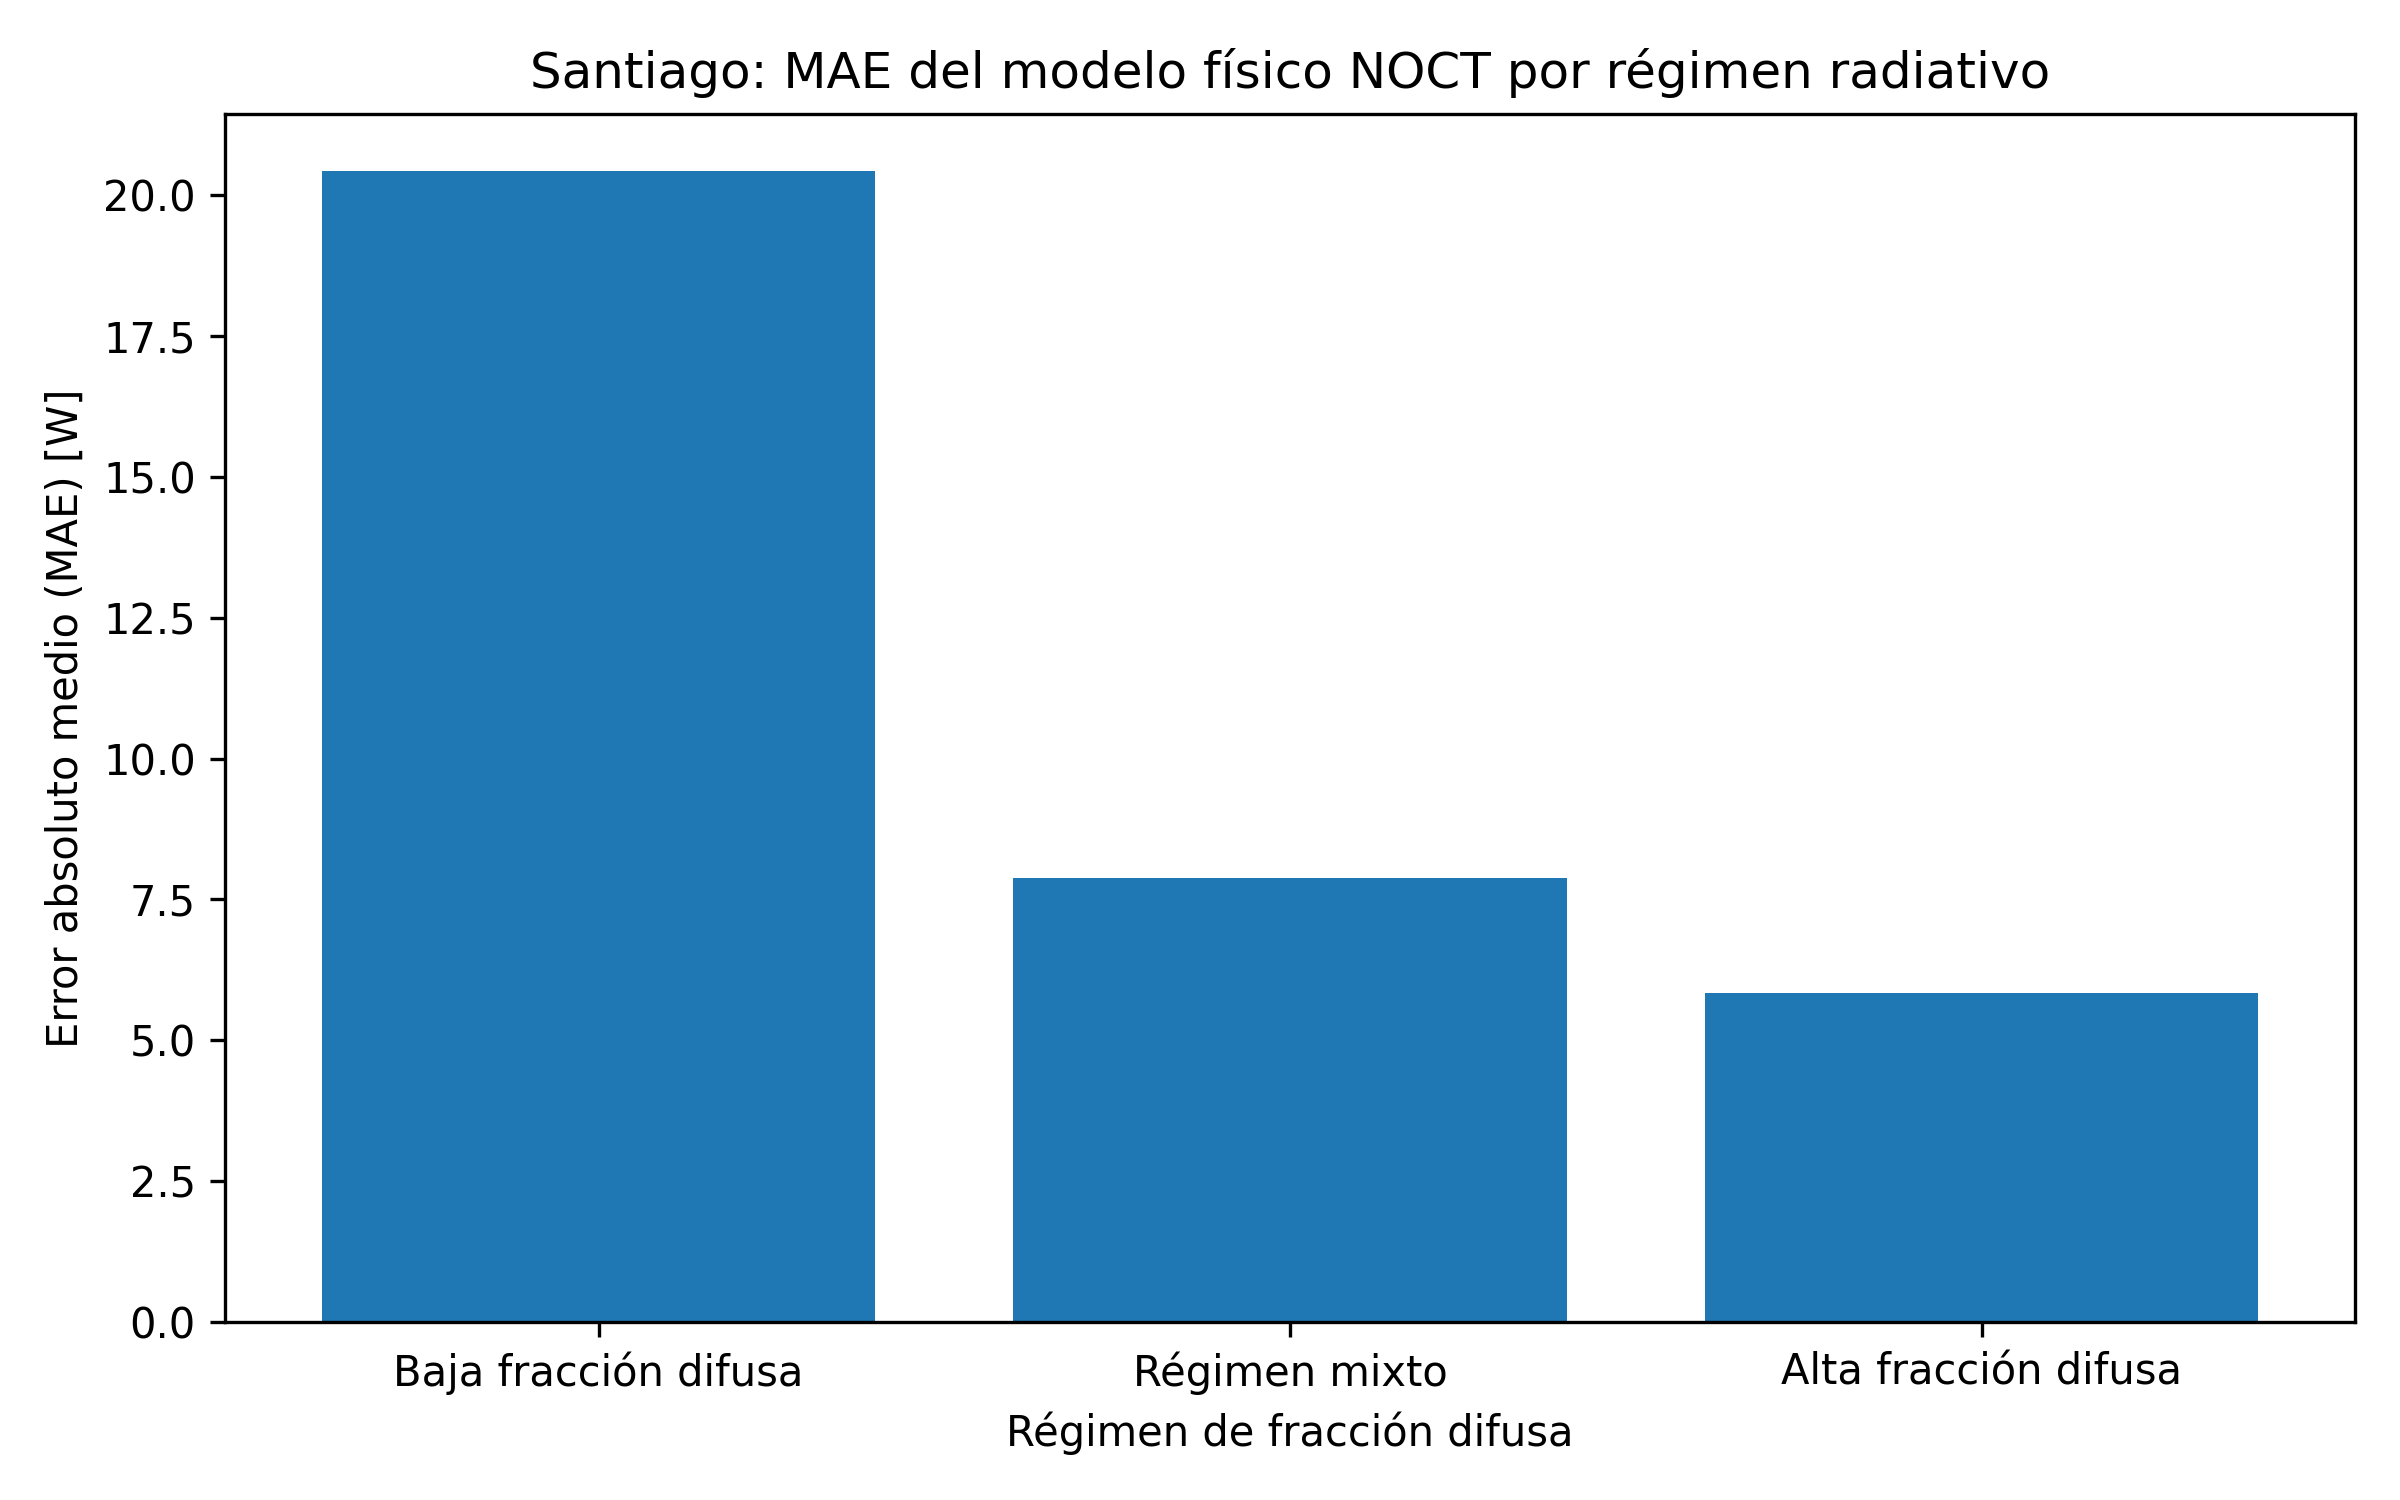
\includegraphics[width=0.82\textwidth]{bar_mae_por_regimen_santiago.png}
    \caption{MAE del modelo NOCT por r\'egimen de fracci\'on difusa para la simulaci\'on asociada a Santiago.}
    \label{fig:mae_regimen}
\end{figure}

\begin{figure}[H]
    \centering
    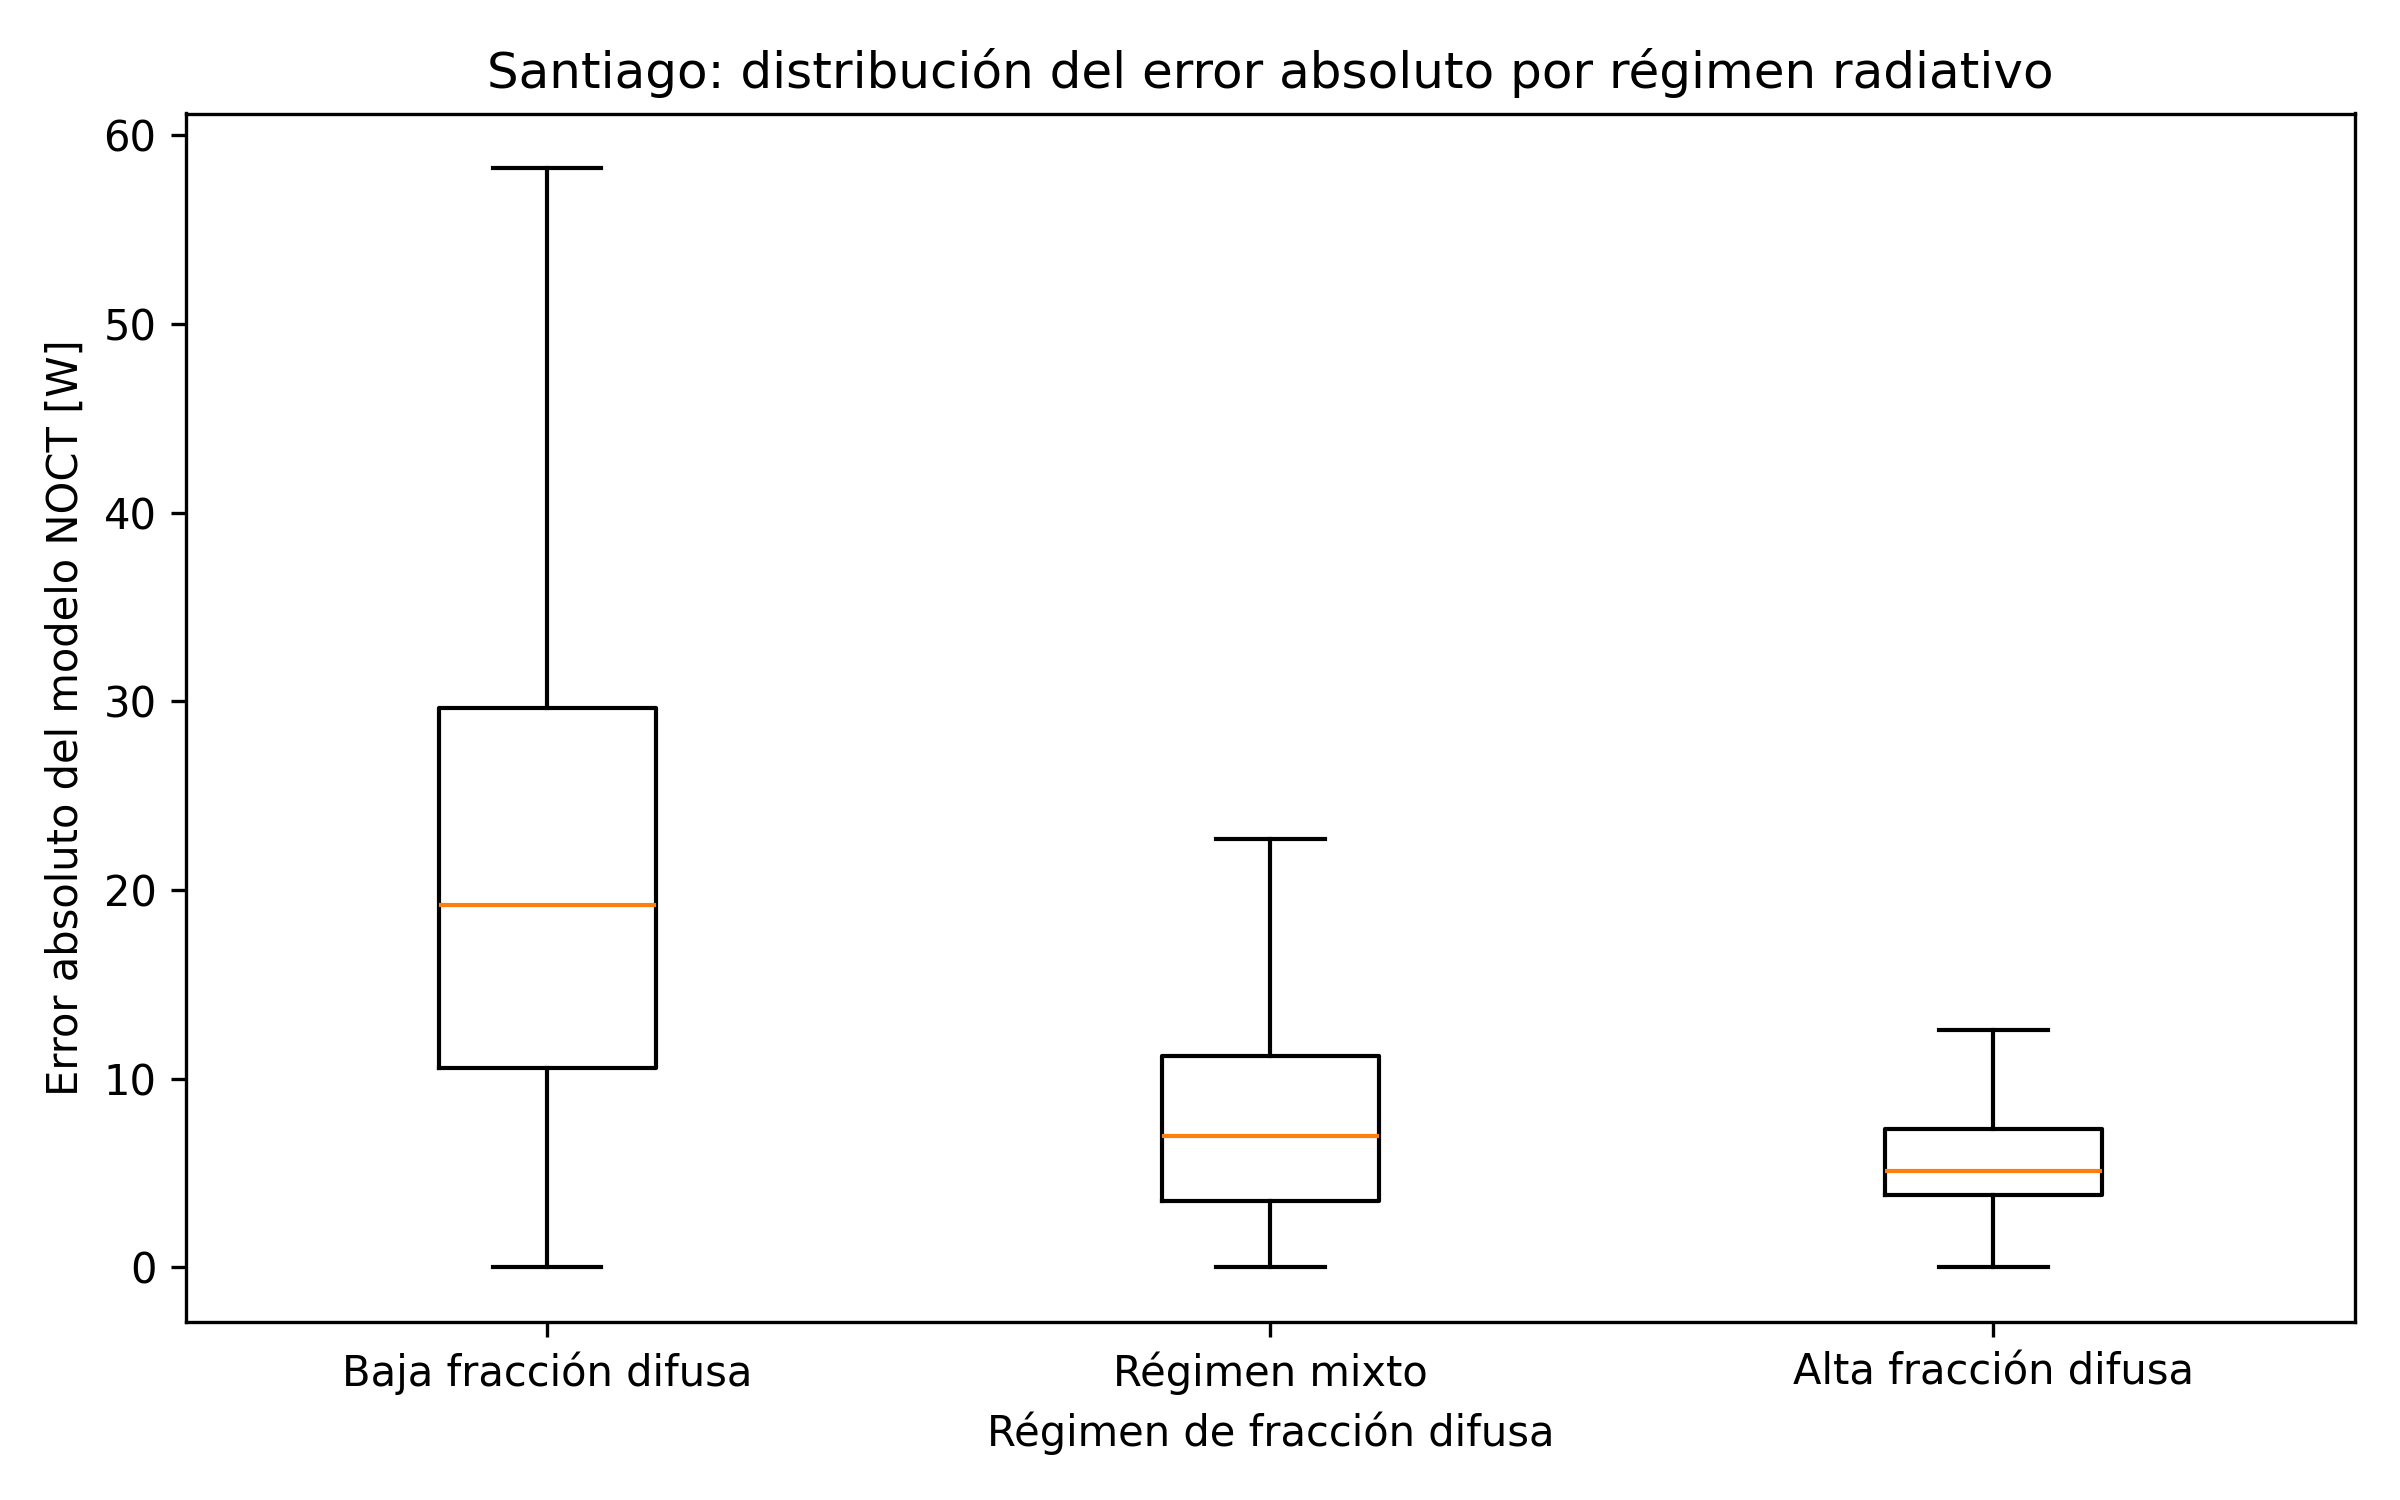
\includegraphics[width=0.82\textwidth]{boxplot_abs_error_por_regimen_santiago.png}
    \caption{Distribuci\'on del error absoluto del modelo NOCT por r\'egimen de fracci\'on difusa; los valores extremos no se muestran en el boxplot.}
    \label{fig:box_abs}
\end{figure}

\subsection{Error relativo por r\'egimen}

Aunque el error absoluto es menor en alta fracci\'on difusa, el error relativo muestra un comportamiento distinto. En condiciones de alta \(fd\), la potencia disponible suele ser menor, por lo que errores absolutos peque\~nos pueden representar una fracci\'on mayor de la potencia generada.

Los resultados indican que el error relativo promedio aumenta en alta fracci\'on difusa, alcanzando aproximadamente 5,15\%. Este resultado es relevante porque sugiere que el desempe\~no proporcional del modelo f\'isico puede degradarse bajo condiciones donde domina la radiaci\'on difusa.

\begin{figure}[H]
    \centering
    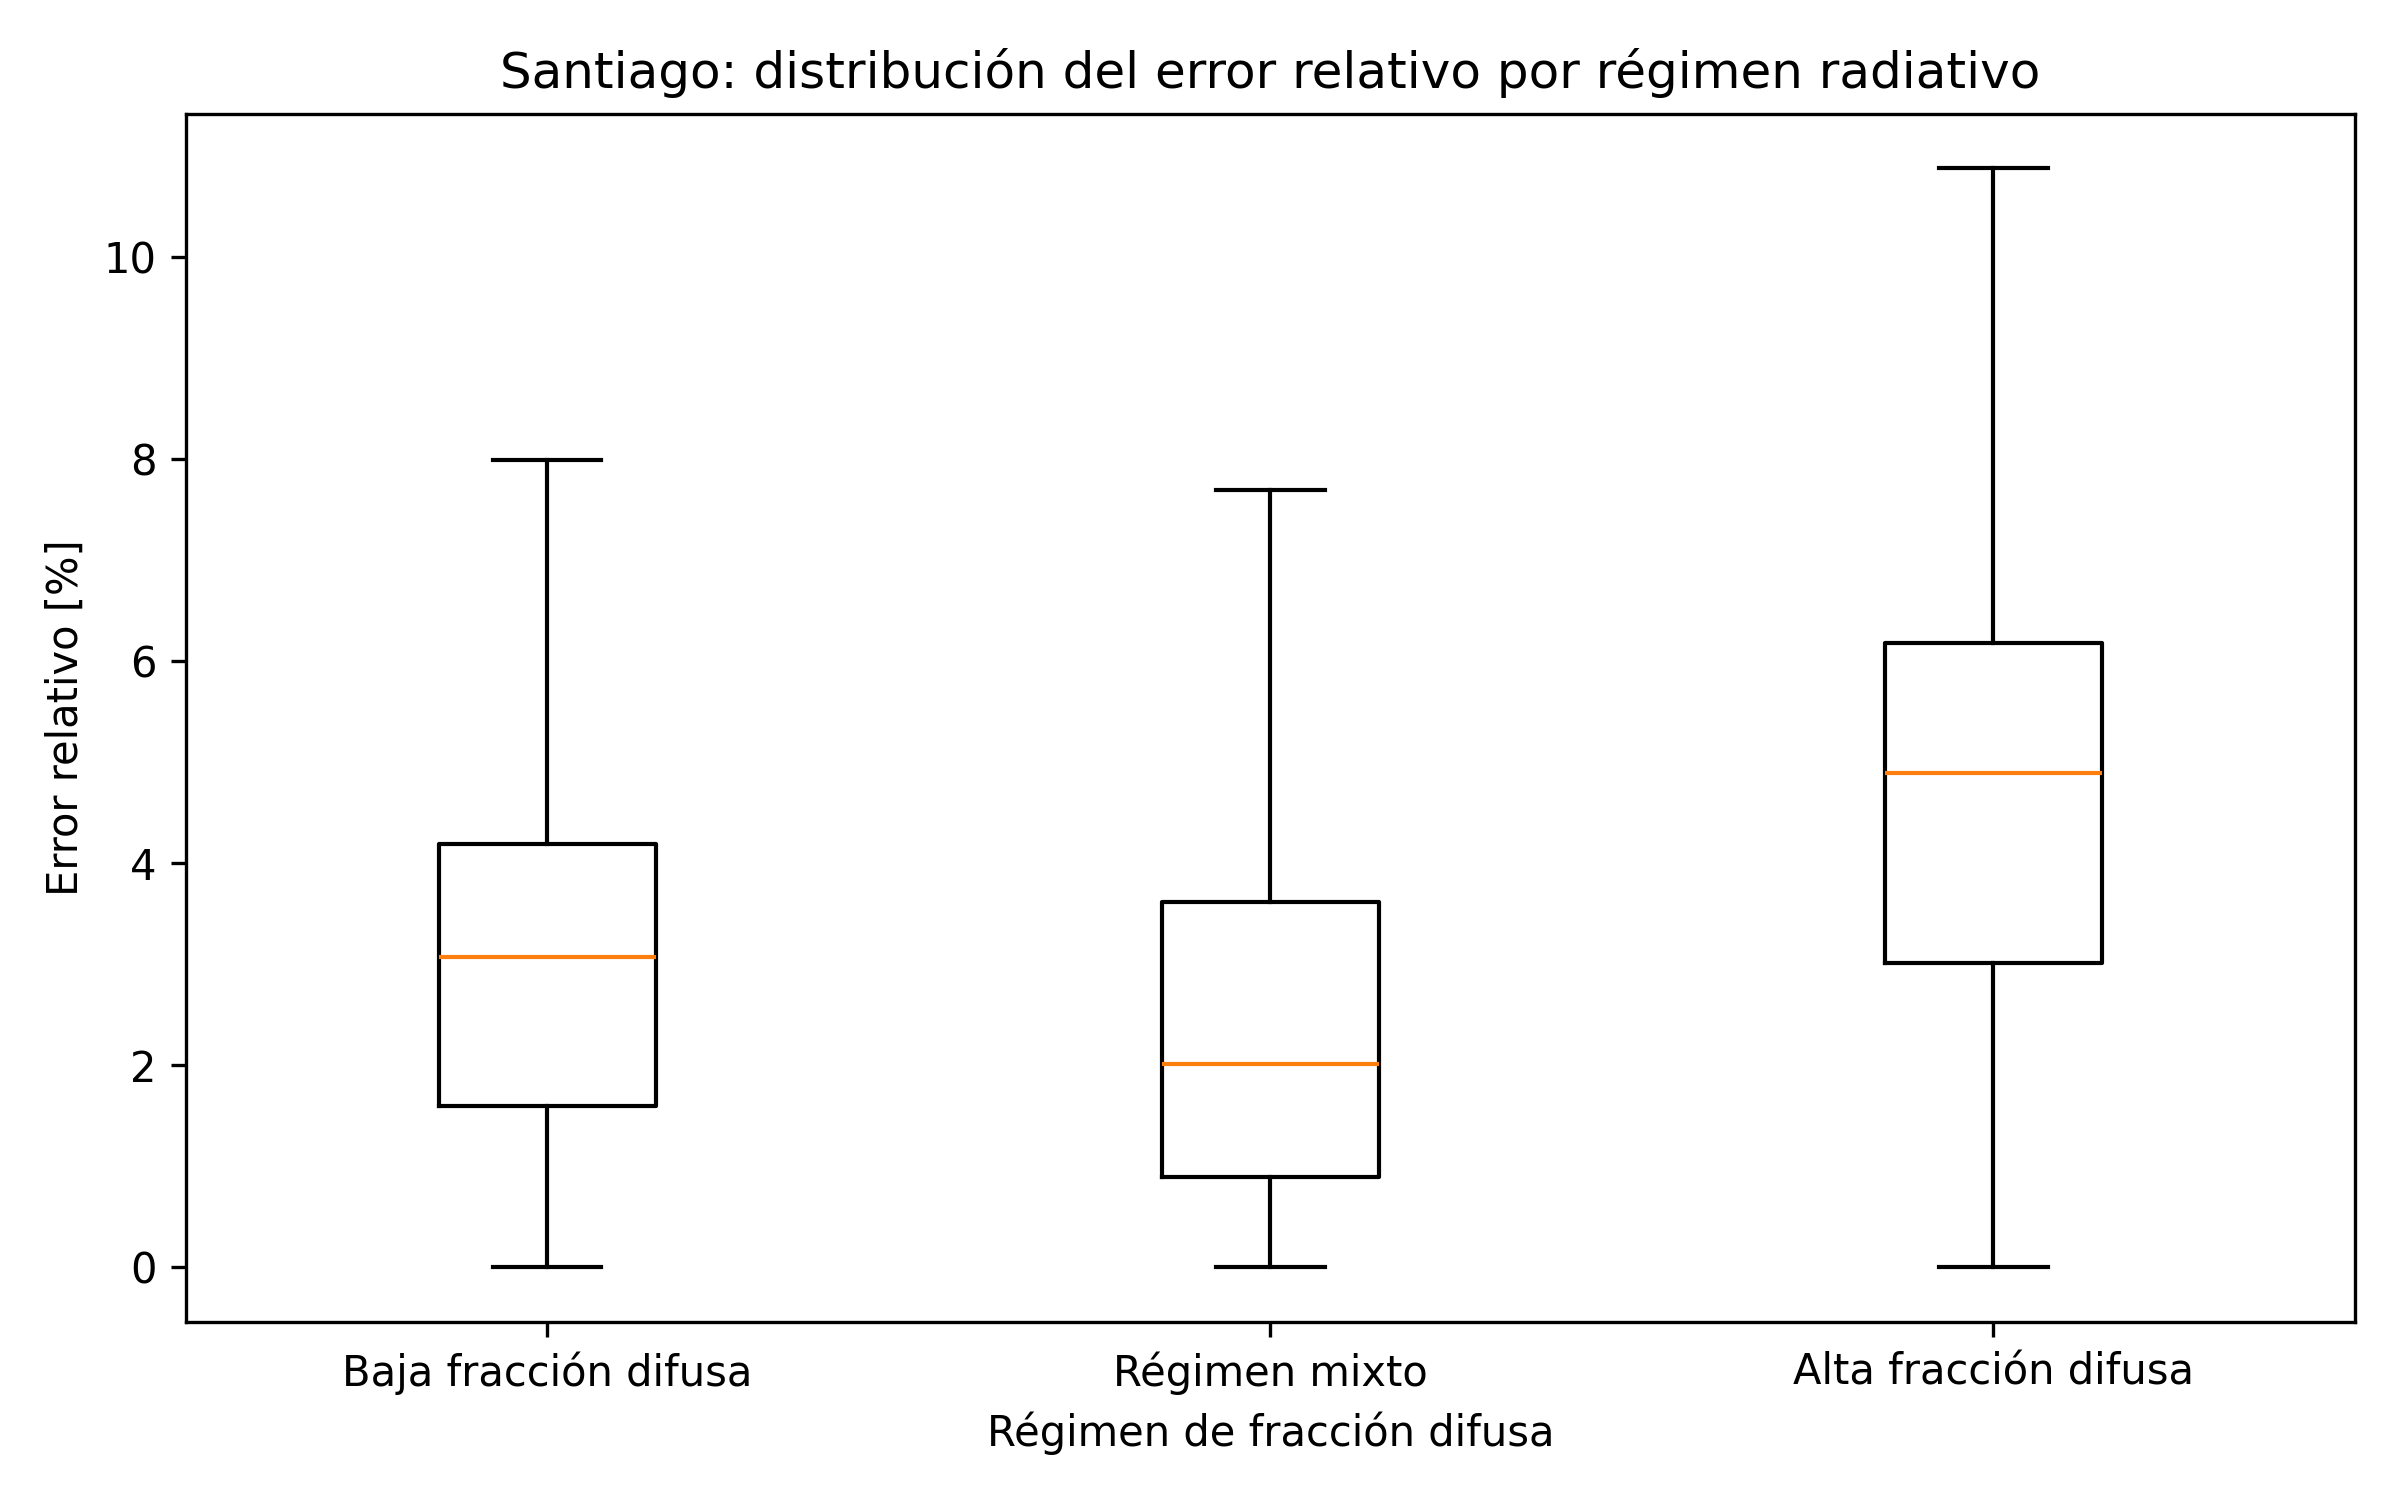
\includegraphics[width=0.82\textwidth]{boxplot_error_relativo_por_regimen_santiago.png}
    \caption{Distribución del error relativo del modelo NOCT por régimen de fracción difusa (los valores extremos no se muestran en el boxplot).}
    \label{fig:box_rel}
\end{figure}

Las Figuras \ref{fig:box_abs} y \ref{fig:box_rel} muestran de este modo que el diagn\'ostico absoluto y el relativo describen aspectos fuertemente complementarios del error.

\subsection{Residuo del modelo NOCT frente a la fracci\'on difusa}

La Figura \ref{fig:epsilon_fd} presenta el residuo \(\epsilon\) frente a \(fd\), lo que permite observar si el error del modelo f\'isico presenta estructura respecto al r\'egimen radiativo. Se observa que el residuo no se distribuye de forma completamente aleatoria, sino que presenta variaciones asociadas a la fracci\'on difusa.

\begin{figure}[H]
    \centering
    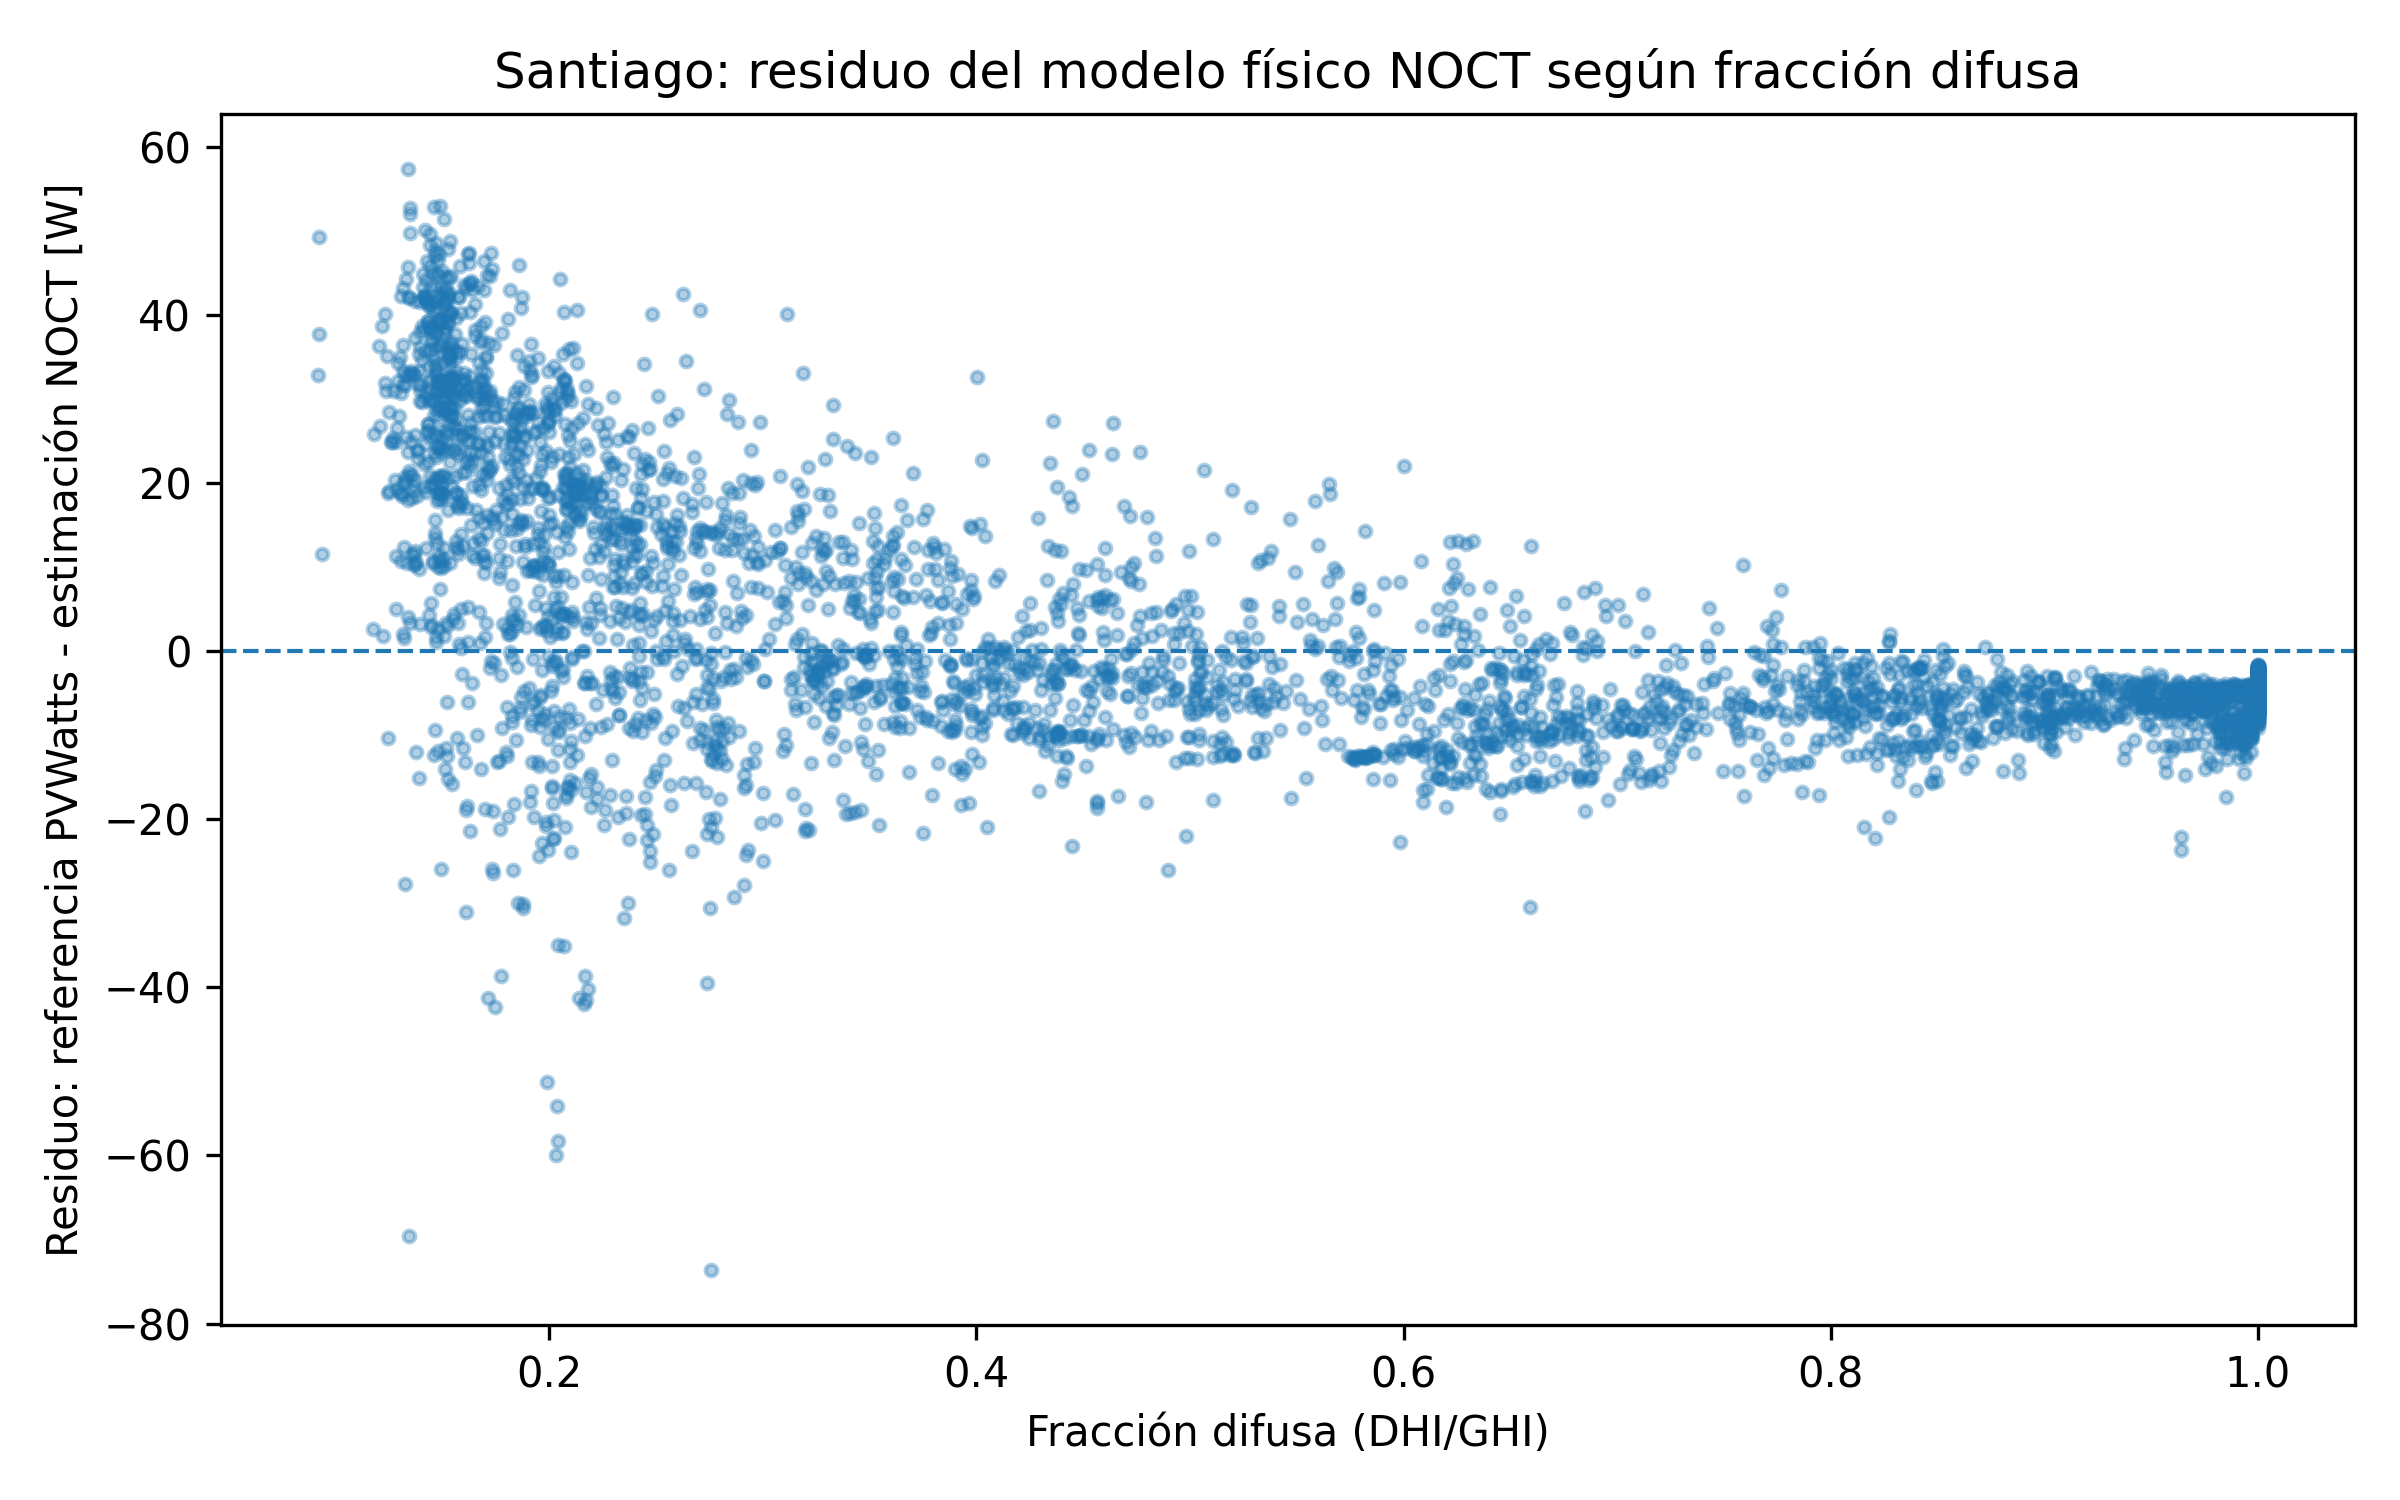
\includegraphics[width=0.86\textwidth]{scatter_epsilon_vs_fd_santiago.png}
    \caption{Residuo del modelo NOCT en funci\'on de la fracci\'on difusa.}
    \label{fig:epsilon_fd}
\end{figure}

Dado que:
\[
    \epsilon = P_{ref} - P_{NOCT},
\]
un residuo negativo indica que el modelo NOCT sobreestima la potencia de referencia, mientras que un residuo positivo indica subestimaci\'on. La observaci\'on de estructura en este gr\'afico justifica la etapa posterior de modelado residual supervisado.

\subsection{Correlaci\'on entre fracci\'on difusa y error}

La Tabla \ref{tab:correlaciones} resume las correlaciones de Pearson y Spearman entre \(fd\) y tres medidas de error. Las correlaciones con \(\epsilon\) y \(|\epsilon|\) se calculan sobre las \(4215\) observaciones válidas. La correlación con error relativo se calcula sobre las \(3688\) observaciones donde dicho error está definido.

\begin{table}[H]
\centering
\caption{Correlaciones entre fracci\'on difusa y medidas de error.}
\label{tab:correlaciones}
\begin{tabular}{lrr}
\toprule
\textbf{Variable de error} & \textbf{Pearson con \(fd\)} & \textbf{Spearman con \(fd\)} \\
\midrule
\(\epsilon\) & -0,5610 & -0,5015 \\
\(|\epsilon|\) & -0,5776 & -0,5729 \\
Error relativo & 0,3591 & 0,3119 \\
\bottomrule
\end{tabular}
\end{table}

Todas las correlaciones presentadas resultaron ser estad\'isticamente significativas (\(p < 0{,}01\)). Es pertinente notar, sin embargo, que las observaciones corresponden a series temporales horarias, donde existe una fuerte autocorrelaci\'on intr\'inseca que puede tender a inflar los niveles de significancia tradicionales. 
Adicionalmente, se detect\'o una alt\'isima colinealidad negativa expl\'icita entre la irradiancia en el plano de arreglo (\(POA\)) y la fracci\'on difusa (\(r = -0{,}8867\)). Esto significa que en condiciones de nubosidad, la p\'erdida de irradiancia total va acoplada fuertemente al aumento en la proporci\'on de irradiancia dispersa.
La correlaci\'on negativa entre \(fd\) y \(\epsilon\) es consistente con el cambio de signo observado en el residuo: bajo baja fracci\'on difusa el modelo tiende a subestimar la referencia simulada, mientras que bajo alta fracci\'on difusa tiende a sobreestimarla. A su vez, la correlaci\'on positiva entre \(fd\) y error relativo indica que el error proporcional tiende a aumentar cuando la fracci\'on difusa es mayor.

\subsection{\texorpdfstring{Comparaci\'on entre \(P_{NOCT}\) y \(P_{ref}\)}{Comparacion entre PNOCT y Pref}}

La comparaci\'on entre la potencia estimada por NOCT y la potencia de referencia simulada por PVWatts, mostrada en la Figura \ref{fig:pnoct_pref}, presenta una alta concordancia global. Esto indica que el modelo f\'isico base entrega una estimaci\'on razonable de la potencia, aunque mantiene errores residuales que pueden ser analizados y eventualmente corregidos.

\begin{figure}[H]
    \centering
    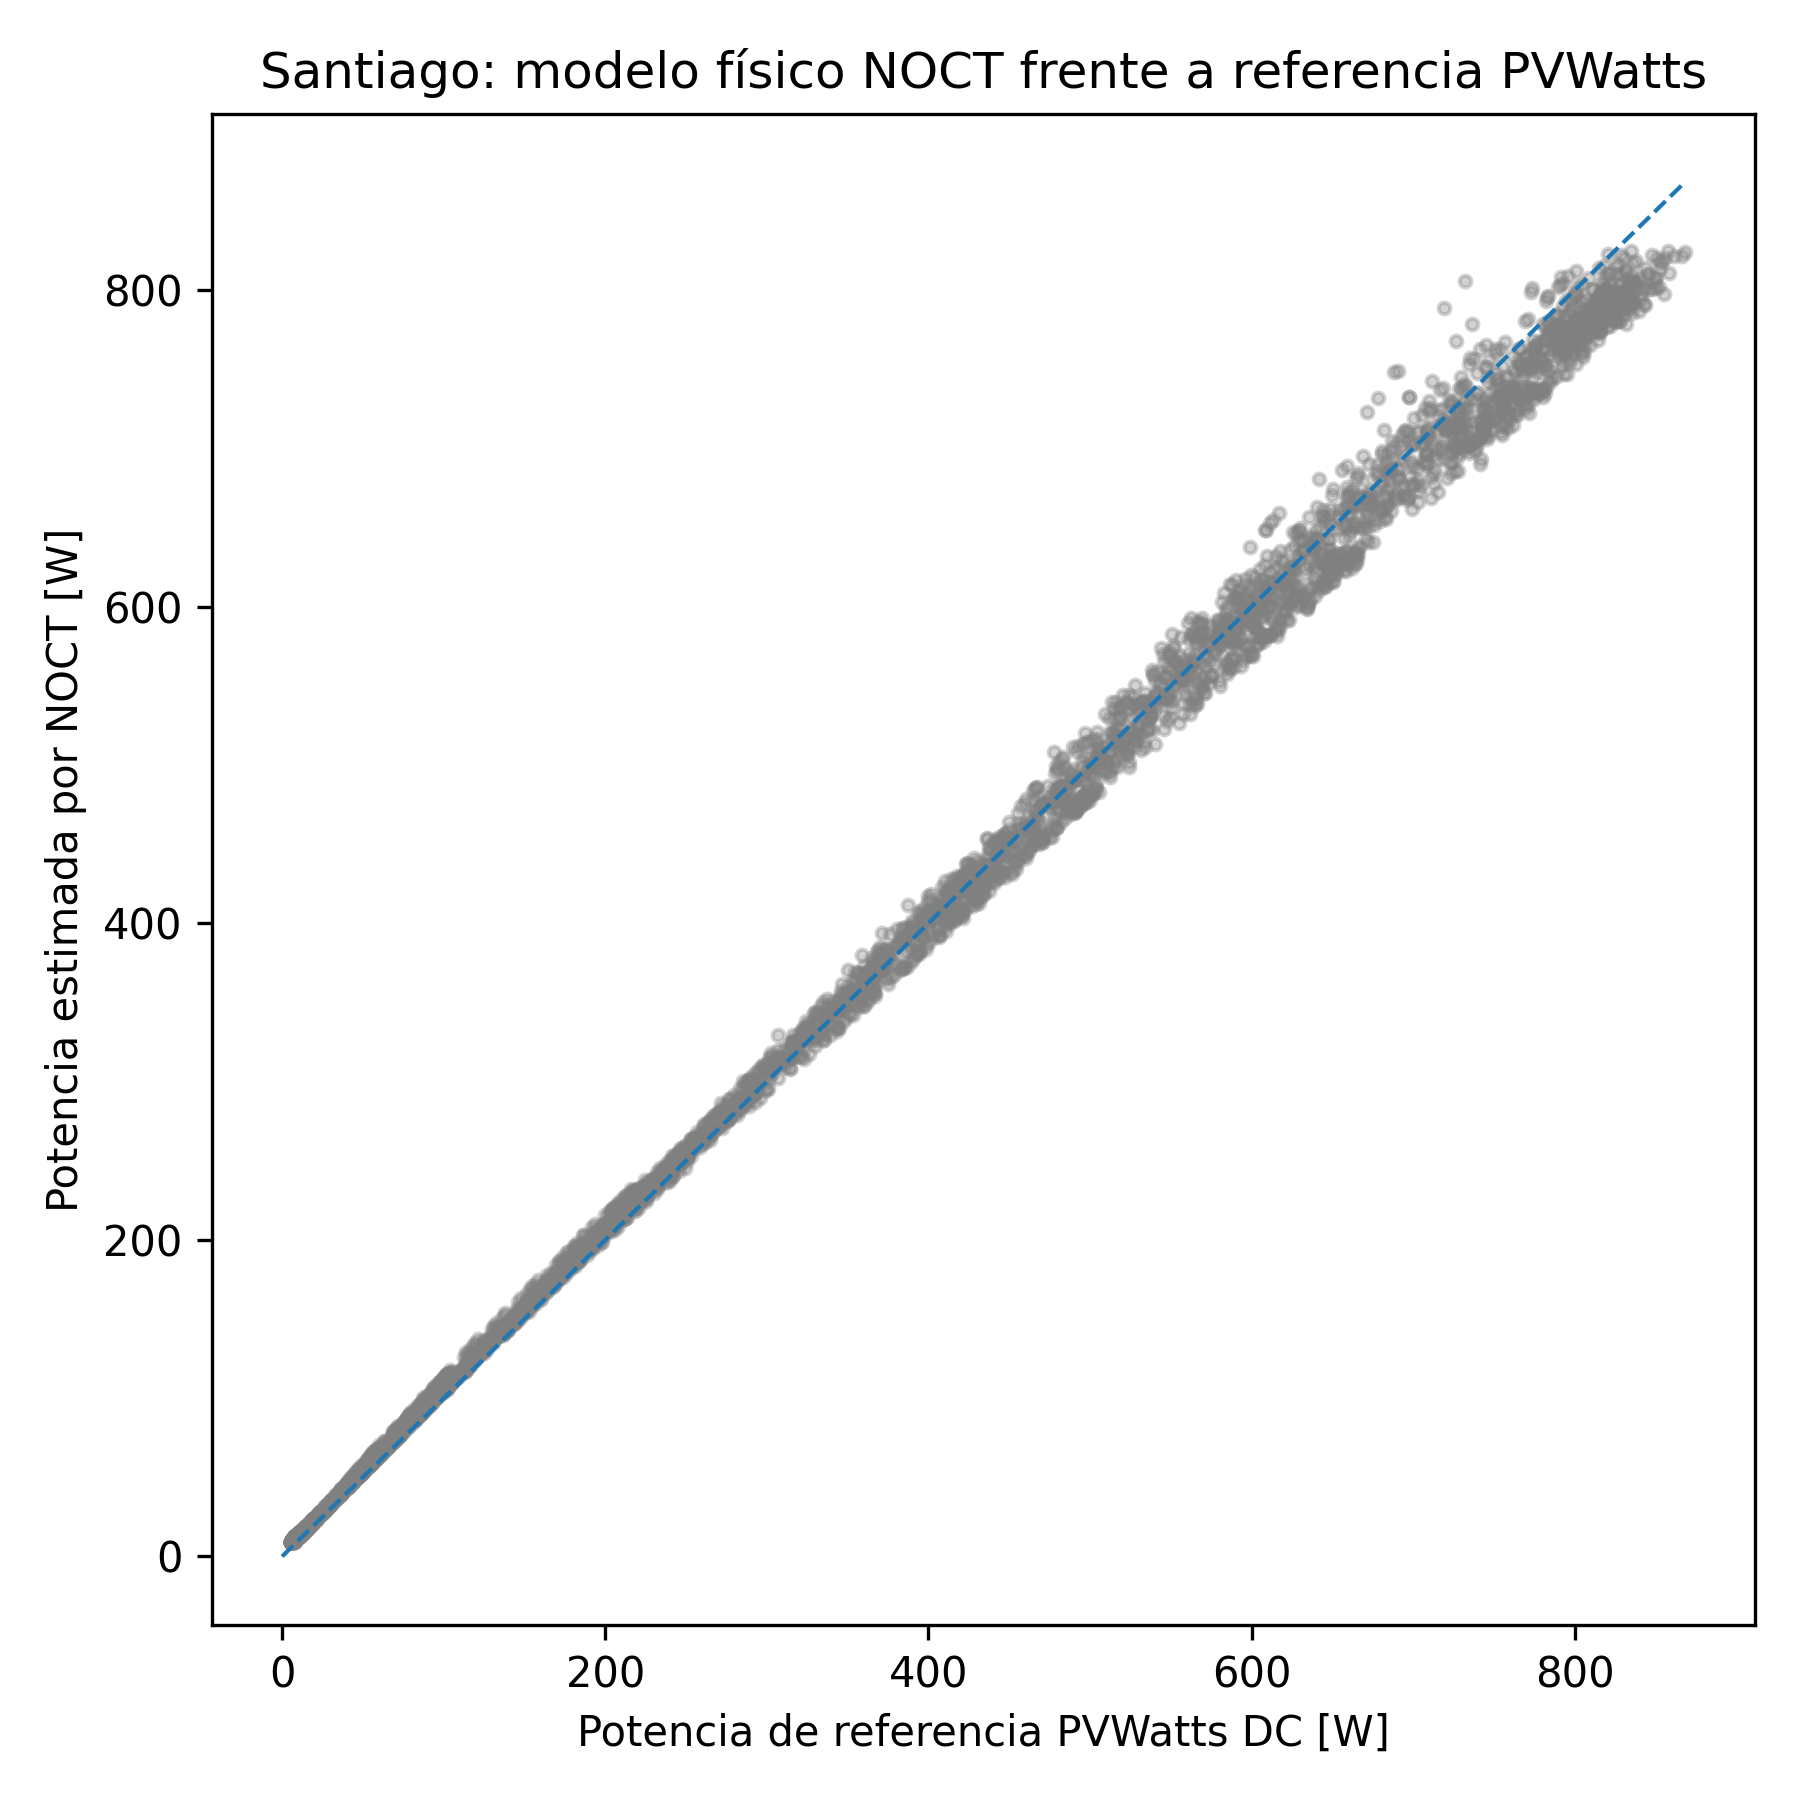
\includegraphics[width=0.76\textwidth]{scatter_pnoct_vs_pref_santiago.png}
    \caption{Comparaci\'on entre potencia estimada por NOCT y potencia de referencia PVWatts.}
    \label{fig:pnoct_pref}
\end{figure}

\subsection{Modelo h\'ibrido residual con XGBoost}

El modelo h\'ibrido utiliza las observaciones v\'alidas para entrenar modelos residuales de XGBoost. La evaluaci\'on principal se realiza con una separaci\'on temporal: el primer 75\% de los datos se utiliza para entrenamiento y el \'ultimo 25\% para prueba. El conjunto de prueba contiene 1054 observaciones v\'alidas, de las cuales 947 tienen error relativo definido bajo el criterio \(P_{ref} > \SI{50}{\watt}\).

La separaci\'on temporal no produce conjuntos clim\'aticamente id\'enticos, lo que es esperable al dividir un a\~no meteorol\'ogico t\'ipico de forma cronol\'ogica. El conjunto de entrenamiento presenta \(fd\) promedio de 0,6070, con 28,69\% de observaciones en baja fracci\'on difusa, 26,38\% en r\'egimen mixto y 44,92\% en alta fracci\'on difusa. En el conjunto de prueba, \(fd\) promedio disminuye a 0,4977 y la proporci\'on de baja fracci\'on difusa aumenta a 41,94\%. Esta diferencia refuerza la necesidad de complementar el holdout final con validaci\'on temporal en m\'ultiples particiones.

Esta etapa debe entenderse como una evaluaci\'on de correcci\'on residual, no como un sistema operacional de pron\'ostico meteorol\'ogico. El modelo aprende a corregir la salida NOCT usando variables disponibles en la misma base horaria simulada y se eval\'ua en un bloque temporal no usado durante el entrenamiento. Por tanto, el objetivo es probar si el residuo contiene estructura aprendible y si \(fd\) aporta informaci\'on adicional, no predecir la radiaci\'on futura a partir de pron\'osticos externos.

La Tabla \ref{tab:metricas_hibrido_test} compara el modelo f\'isico NOCT con dos versiones del modelo h\'ibrido: una sin fracci\'on difusa y otra incorporando expl\'icitamente la fracci\'on difusa. En ambos casos, XGBoost aprende el residuo \(\epsilon\) y la potencia final se calcula como \(P_{hybrid}=P_{NOCT}+\widehat{\epsilon}\).

Esta forma de evaluación permite separar dos preguntas. La primera es si el residuo del modelo físico contiene patrones aprendibles usando variables meteorológicas y temporales. Esta pregunta se responde comparando NOCT contra el modelo híbrido sin \(fd\). La segunda es si la fracción difusa agrega información adicional. Esta pregunta se responde comparando el híbrido sin \(fd\) contra el híbrido con \(fd\). Por ello, la evidencia no depende solo de que XGBoost mejore a NOCT, sino de que la versión con \(fd\) mejore a una versión equivalente sin esa variable.

\begin{table}[H]
\centering
\caption{Desempe\~no de los modelos en el conjunto temporal de prueba.}
\label{tab:metricas_hibrido_test}
\small
\resizebox{\textwidth}{!}{%
\begin{tabular}{lrrrrr}
\toprule
\textbf{Modelo} & \textbf{MAE [W]} & \textbf{RMSE [W]} & \textbf{Bias [W]} & \textbf{Error rel. [\%]} & \textbf{Mejora MAE [\%]} \\
\midrule
Modelo f\'isico NOCT & 13,30 & 17,10 & -4,05 & 3,96 & 0,00 \\
H\'ibrido sin fracci\'on difusa & 2,70 & 3,73 & 0,92 & 0,94 & 79,67 \\
H\'ibrido con fracci\'on difusa & 2,22 & 3,01 & 1,13 & 0,83 & 83,27 \\
\bottomrule
\end{tabular}%
}
\end{table}

El modelo h\'ibrido sin fracci\'on difusa reduce el MAE desde \SI{13.30}{\watt} hasta \SI{2.70}{\watt}, lo que muestra que el residuo del modelo NOCT contiene estructura aprendible a partir de variables f\'isicas y temporales. Al incorporar la fracci\'on difusa, el MAE disminuye adicionalmente hasta \SI{2.22}{\watt}. Esto corresponde a una mejora de 83,27\% respecto al modelo f\'isico NOCT y a una mejora adicional de aproximadamente 17,69\% respecto al h\'ibrido sin fracci\'on difusa.

El hecho de que el modelo sin \(fd\) ya reduzca fuertemente el error indica que parte de la discrepancia entre NOCT y PVWatts est\'a asociada a variables generales del estado operativo del sistema, como irradiancia en el plano del panel, temperatura, viento y ciclos horarios o estacionales. La mejora adicional al incluir \(fd\) indica que, aun despu\'es de considerar esas variables, la composici\'on directa--difusa de la irradiancia conserva informaci\'on predictiva sobre el residuo.

La Tabla \ref{tab:train_test_hibrido} compara el desempe\~no en entrenamiento y prueba. Como es esperable, los modelos supervisados presentan menor error en entrenamiento que en prueba. No obstante, la mejora respecto al NOCT se mantiene en el conjunto temporal no usado para entrenar, lo que indica que el resultado no corresponde solo a ajuste sobre los datos de entrenamiento.

\begin{table}[H]
\centering
\caption{Comparaci\'on de MAE y RMSE en entrenamiento y prueba.}
\label{tab:train_test_hibrido}
\resizebox{\textwidth}{!}{%
\begin{tabular}{llrrr}
\toprule
\textbf{Conjunto} & \textbf{Modelo} & \textbf{MAE [W]} & \textbf{RMSE [W]} & \textbf{Mejora MAE [\%]} \\
\midrule
Entrenamiento & Modelo f\'isico NOCT & 10,30 & 14,30 & 0,00 \\
Entrenamiento & H\'ibrido sin fracci\'on difusa & 1,46 & 2,02 & 85,82 \\
Entrenamiento & H\'ibrido con fracci\'on difusa & 1,11 & 1,49 & 89,24 \\
Prueba & Modelo f\'isico NOCT & 13,30 & 17,10 & 0,00 \\
Prueba & H\'ibrido sin fracci\'on difusa & 2,70 & 3,73 & 79,67 \\
Prueba & H\'ibrido con fracci\'on difusa & 2,22 & 3,01 & 83,27 \\
\bottomrule
\end{tabular}%
}
\end{table}

La diferencia entre entrenamiento y prueba se interpreta como una verificaci\'on de generalizaci\'on. Si el modelo h\'ibrido solo estuviera memorizando los datos de entrenamiento, se esperar\'ia una mejora grande en entrenamiento y una p\'erdida marcada de desempe\~no en prueba. En cambio, aunque el error aumenta al pasar al bloque temporal de prueba, el MAE se mantiene muy por debajo del NOCT base. Esto sugiere que el modelo residual aprende patrones persistentes del error f\'isico y no solamente fluctuaciones particulares del conjunto de entrenamiento. La Figura \ref{fig:mae_modelos_test} resume la reducci\'on de MAE en el conjunto de prueba.

\begin{figure}[H]
    \centering
    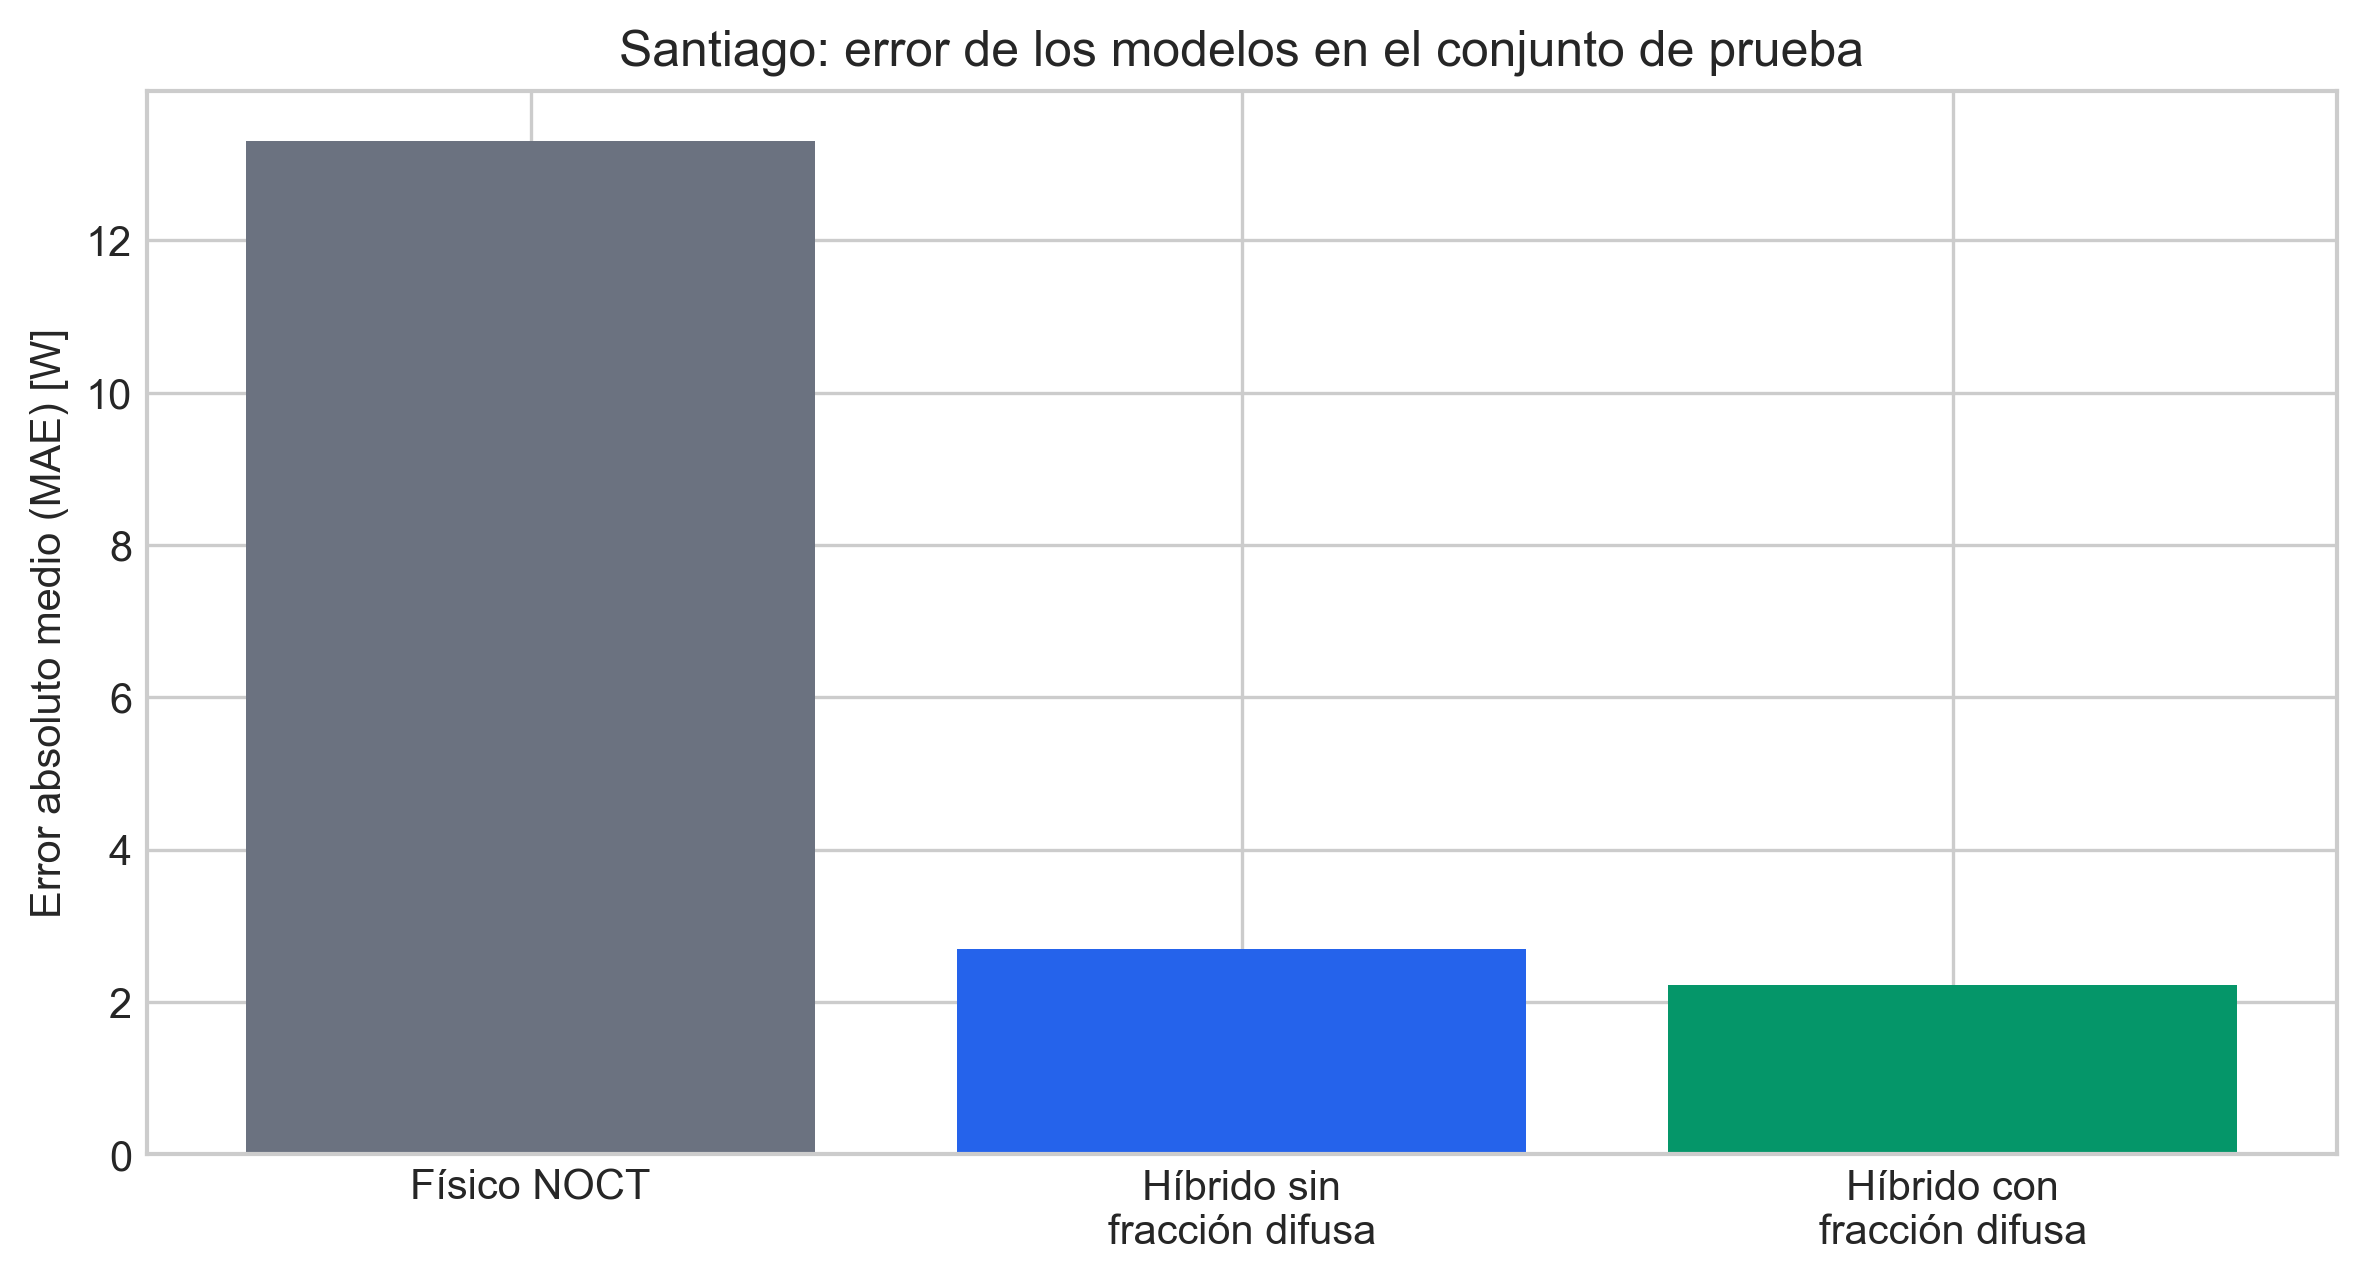
\includegraphics[width=0.82\textwidth]{bar_mae_modelos_test_santiago.png}
    \caption{Comparaci\'on del MAE entre el modelo f\'isico NOCT y los modelos h\'ibridos en el conjunto de prueba.}
    \label{fig:mae_modelos_test}
\end{figure}

\subsection{Desempe\~no del modelo h\'ibrido por r\'egimen}

La Tabla \ref{tab:metricas_hibrido_regimen} muestra el MAE de cada modelo separado por r\'egimen de fracci\'on difusa. La mejora del modelo h\'ibrido con fracci\'on difusa se observa en los tres reg\'imenes, aunque su magnitud absoluta depende del nivel de error inicial del modelo NOCT.

\begin{table}[H]
\centering
\caption{MAE por r\'egimen de fracci\'on difusa en el conjunto temporal de prueba.}
\label{tab:metricas_hibrido_regimen}
\resizebox{\textwidth}{!}{%
\begin{tabular}{lrrrr}
\toprule
\textbf{R\'egimen} & \textbf{NOCT [W]} & \textbf{H\'ibrido sin fracci\'on difusa [W]} & \textbf{H\'ibrido con fracci\'on difusa [W]} & \textbf{Mejora con \(fd\) vs. NOCT [\%]} \\
\midrule
Baja fracci\'on difusa & 21,13 & 2,34 & 2,03 & 90,40 \\
Mixto & 9,27 & 3,33 & 2,95 & 68,14 \\
Alta fracci\'on difusa & 6,16 & 2,64 & 1,83 & 70,23 \\
\bottomrule
\end{tabular}%
}
\end{table}

En baja fracci\'on difusa, donde el modelo NOCT presentaba el mayor error absoluto, el h\'ibrido con fracci\'on difusa reduce el MAE desde \SI{21.13}{\watt} hasta \SI{2.03}{\watt}. En alta fracci\'on difusa, donde el error relativo del NOCT era m\'as alto, el MAE disminuye desde \SI{6.16}{\watt} hasta \SI{1.83}{\watt}. Por tanto, la correcci\'on residual mejora tanto las condiciones de mayor potencia como aquellas donde la componente difusa domina. La Figura \ref{fig:mae_modelos_regimen} permite comparar visualmente esta reducci\'on por r\'egimen.

\begin{figure}[H]
    \centering
    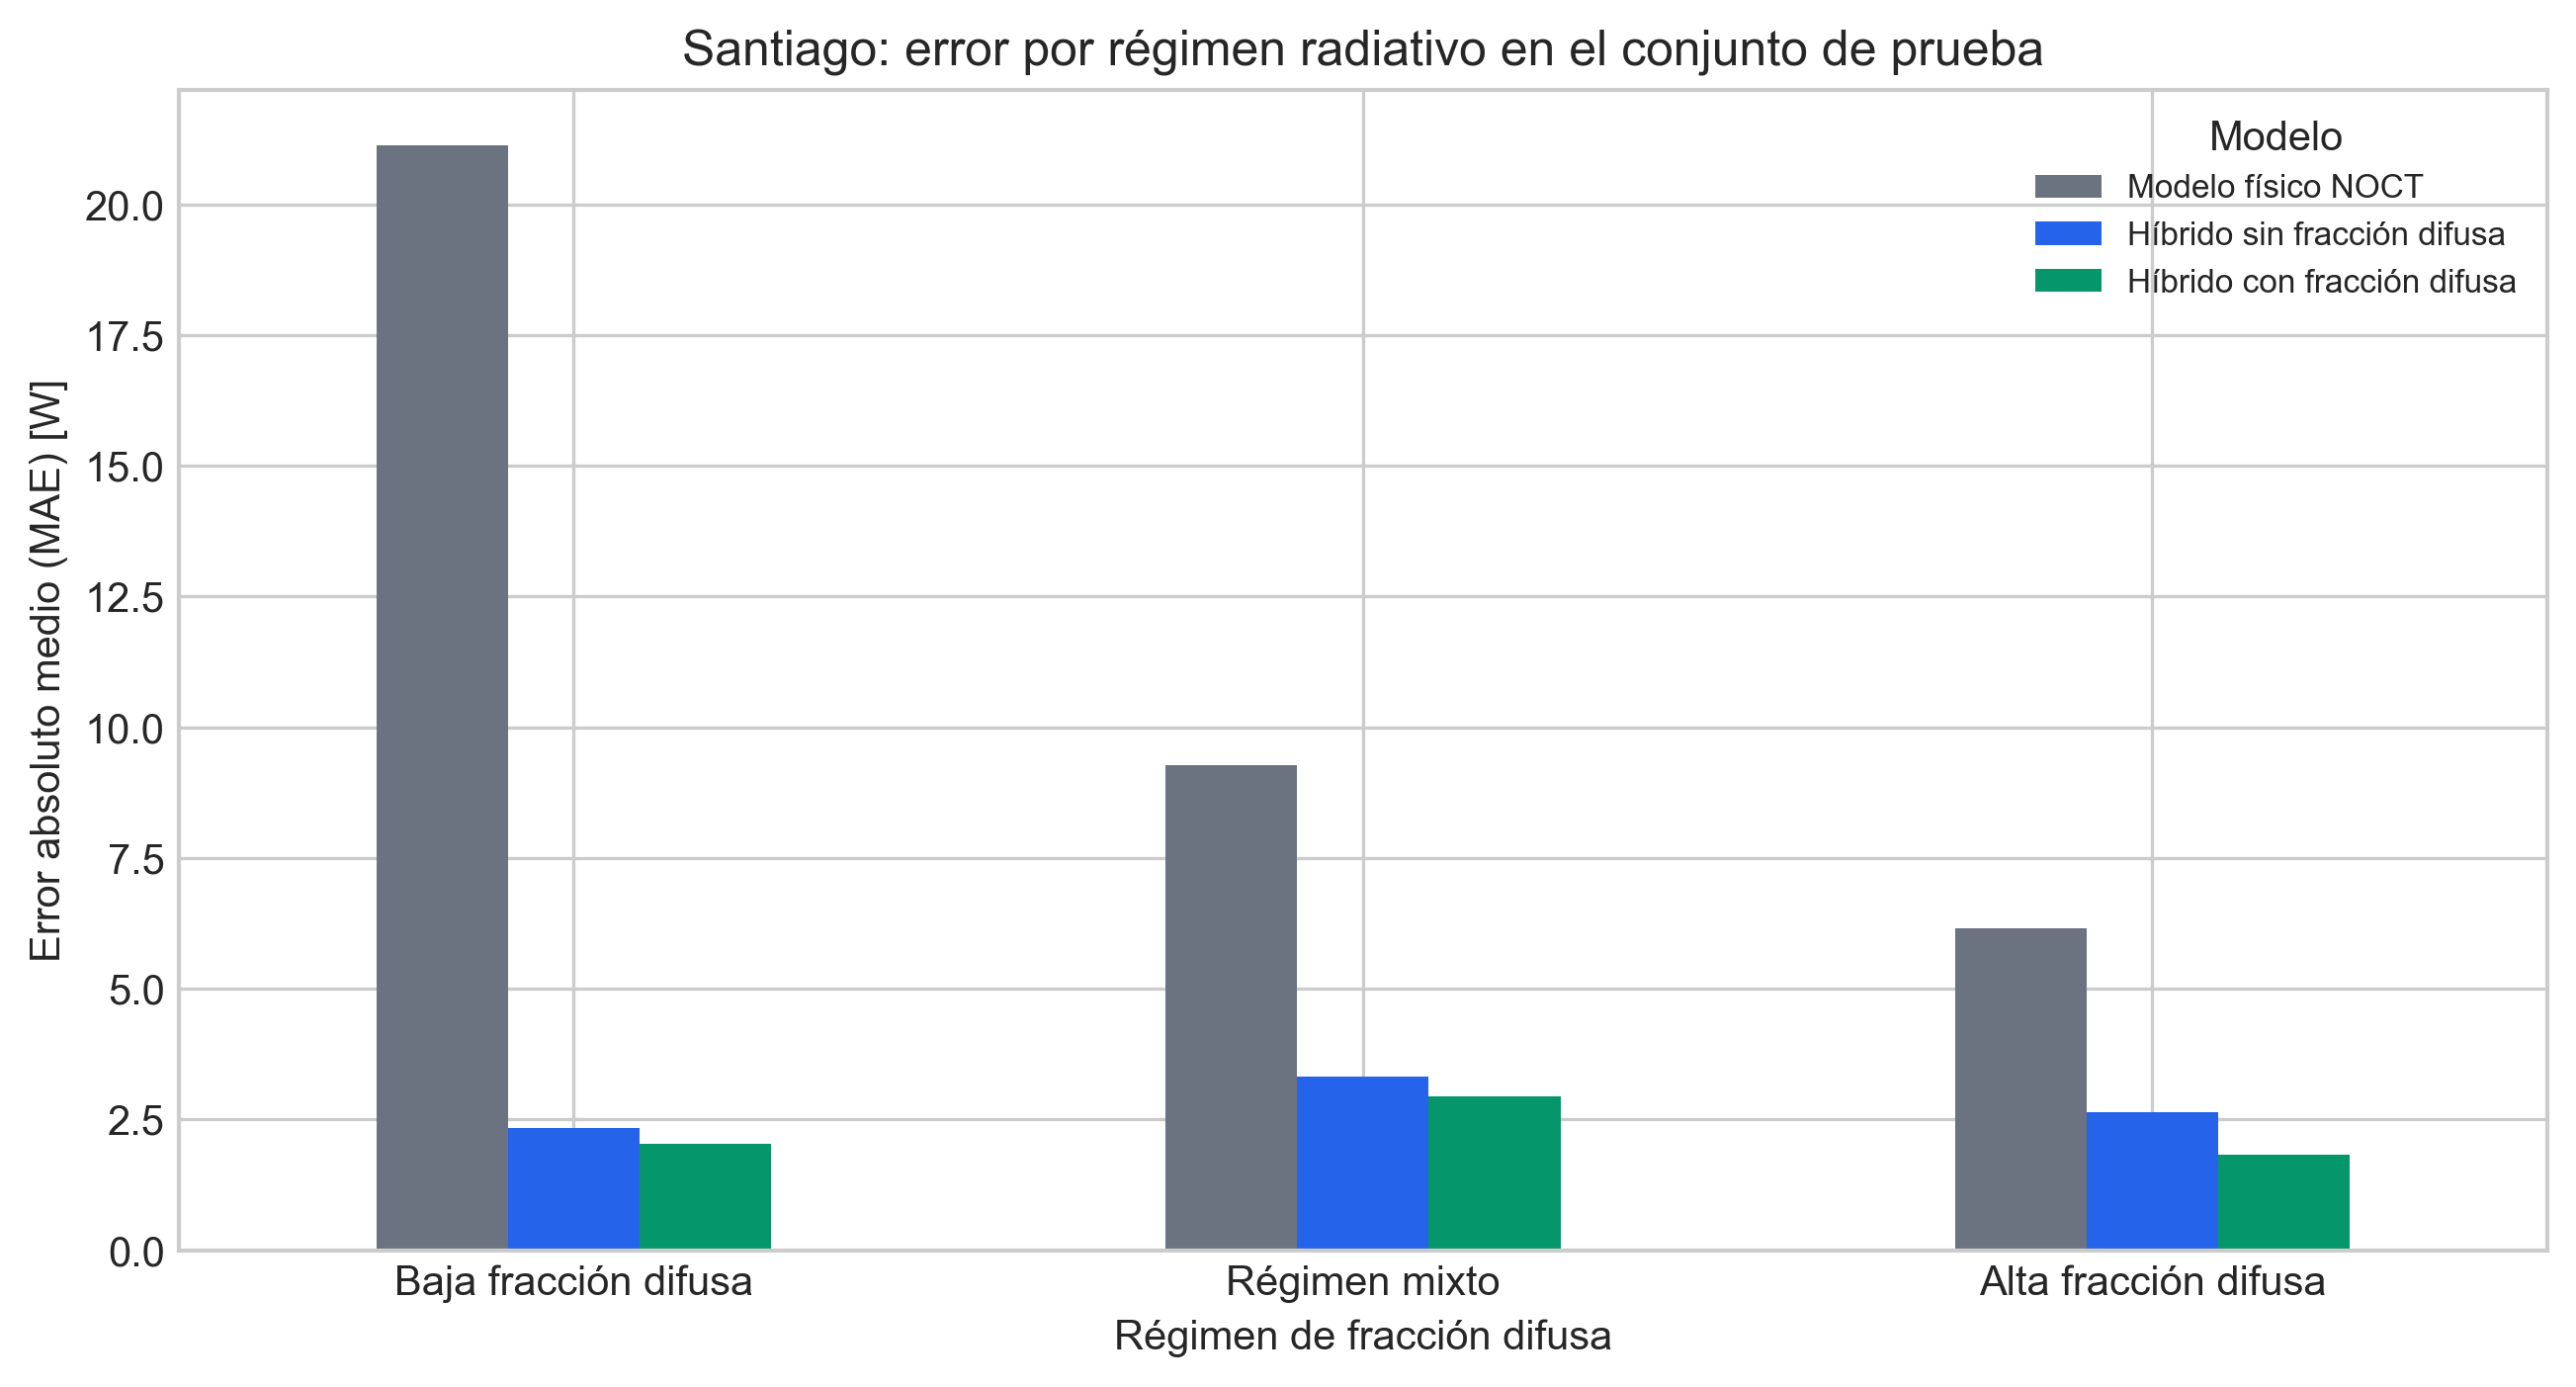
\includegraphics[width=0.84\textwidth]{bar_mae_por_regimen_modelos_santiago.png}
    \caption{MAE del modelo f\'isico NOCT y de los modelos h\'ibridos por r\'egimen de fracci\'on difusa.}
    \label{fig:mae_modelos_regimen}
\end{figure}

\subsection{Residuo corregido e importancia de variables}

La Figura \ref{fig:residuo_fd_hibrido} compara el residuo del modelo NOCT con el residuo del modelo h\'ibrido con fracci\'on difusa en el conjunto de prueba. La dispersi\'on residual disminuye de forma visible, lo que es consistente con la reducci\'on de MAE y RMSE reportada en la Tabla \ref{tab:metricas_hibrido_test}.

\begin{figure}[H]
    \centering
    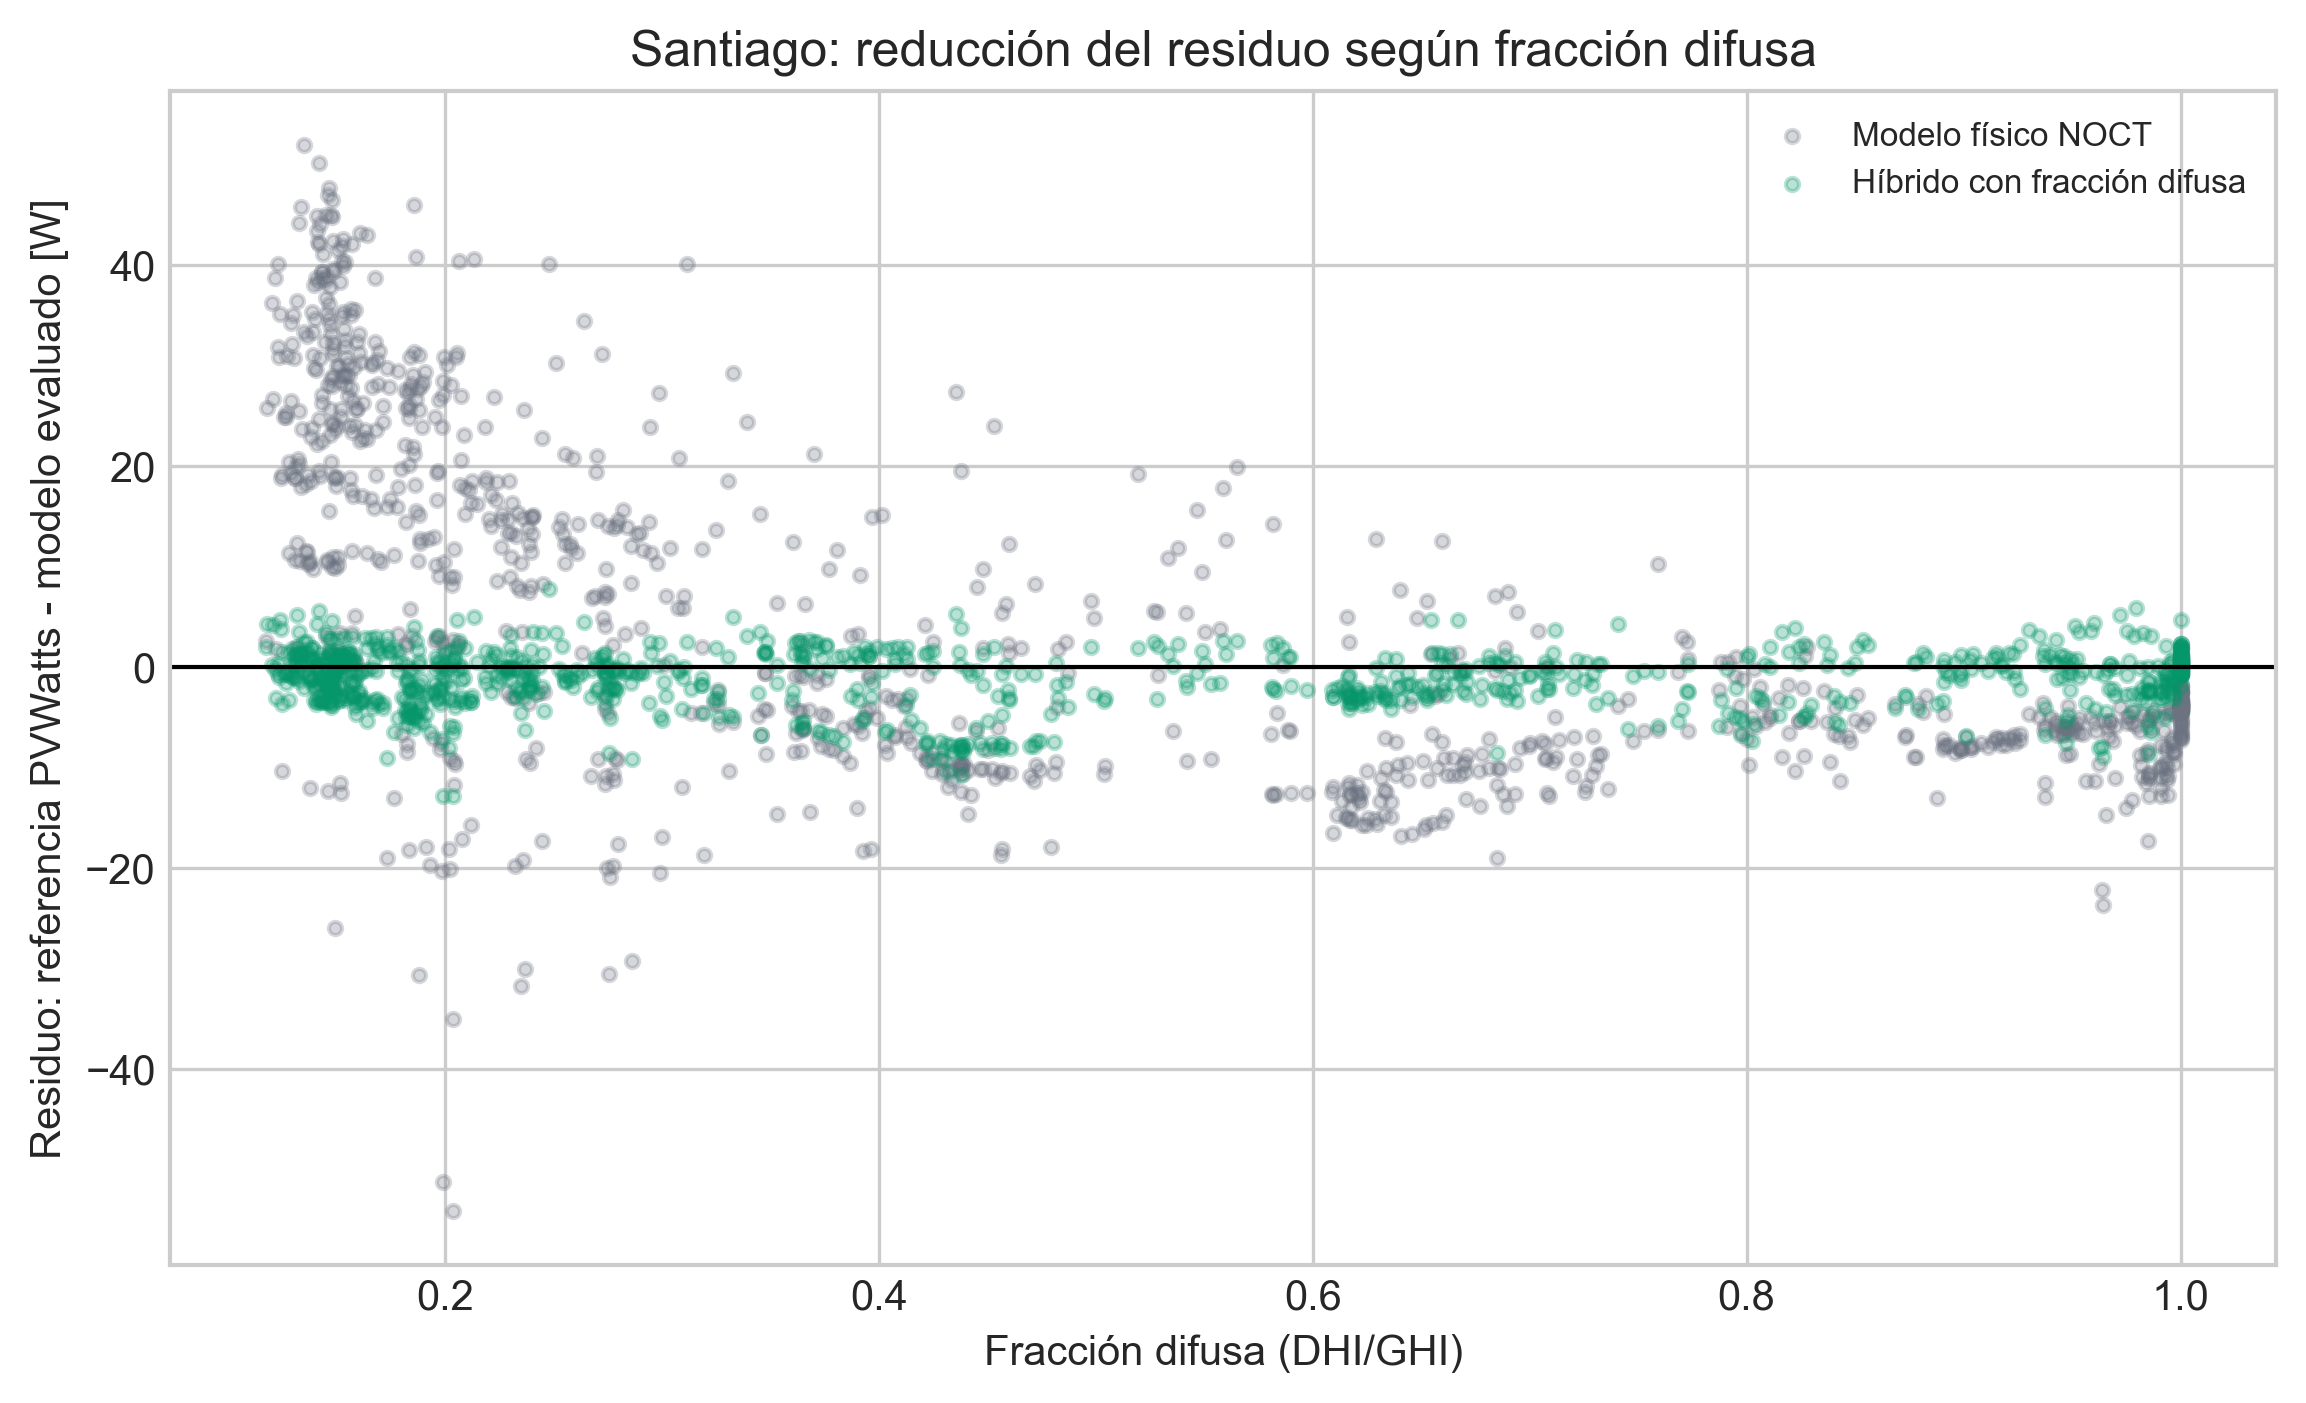
\includegraphics[width=0.86\textwidth]{scatter_residuo_vs_fd_noct_hibrido_santiago.png}
    \caption{Residuo del modelo f\'isico NOCT y del modelo h\'ibrido con fracci\'on difusa frente a la fracci\'on difusa.}
    \label{fig:residuo_fd_hibrido}
\end{figure}

\begin{figure}[H]
    \centering
    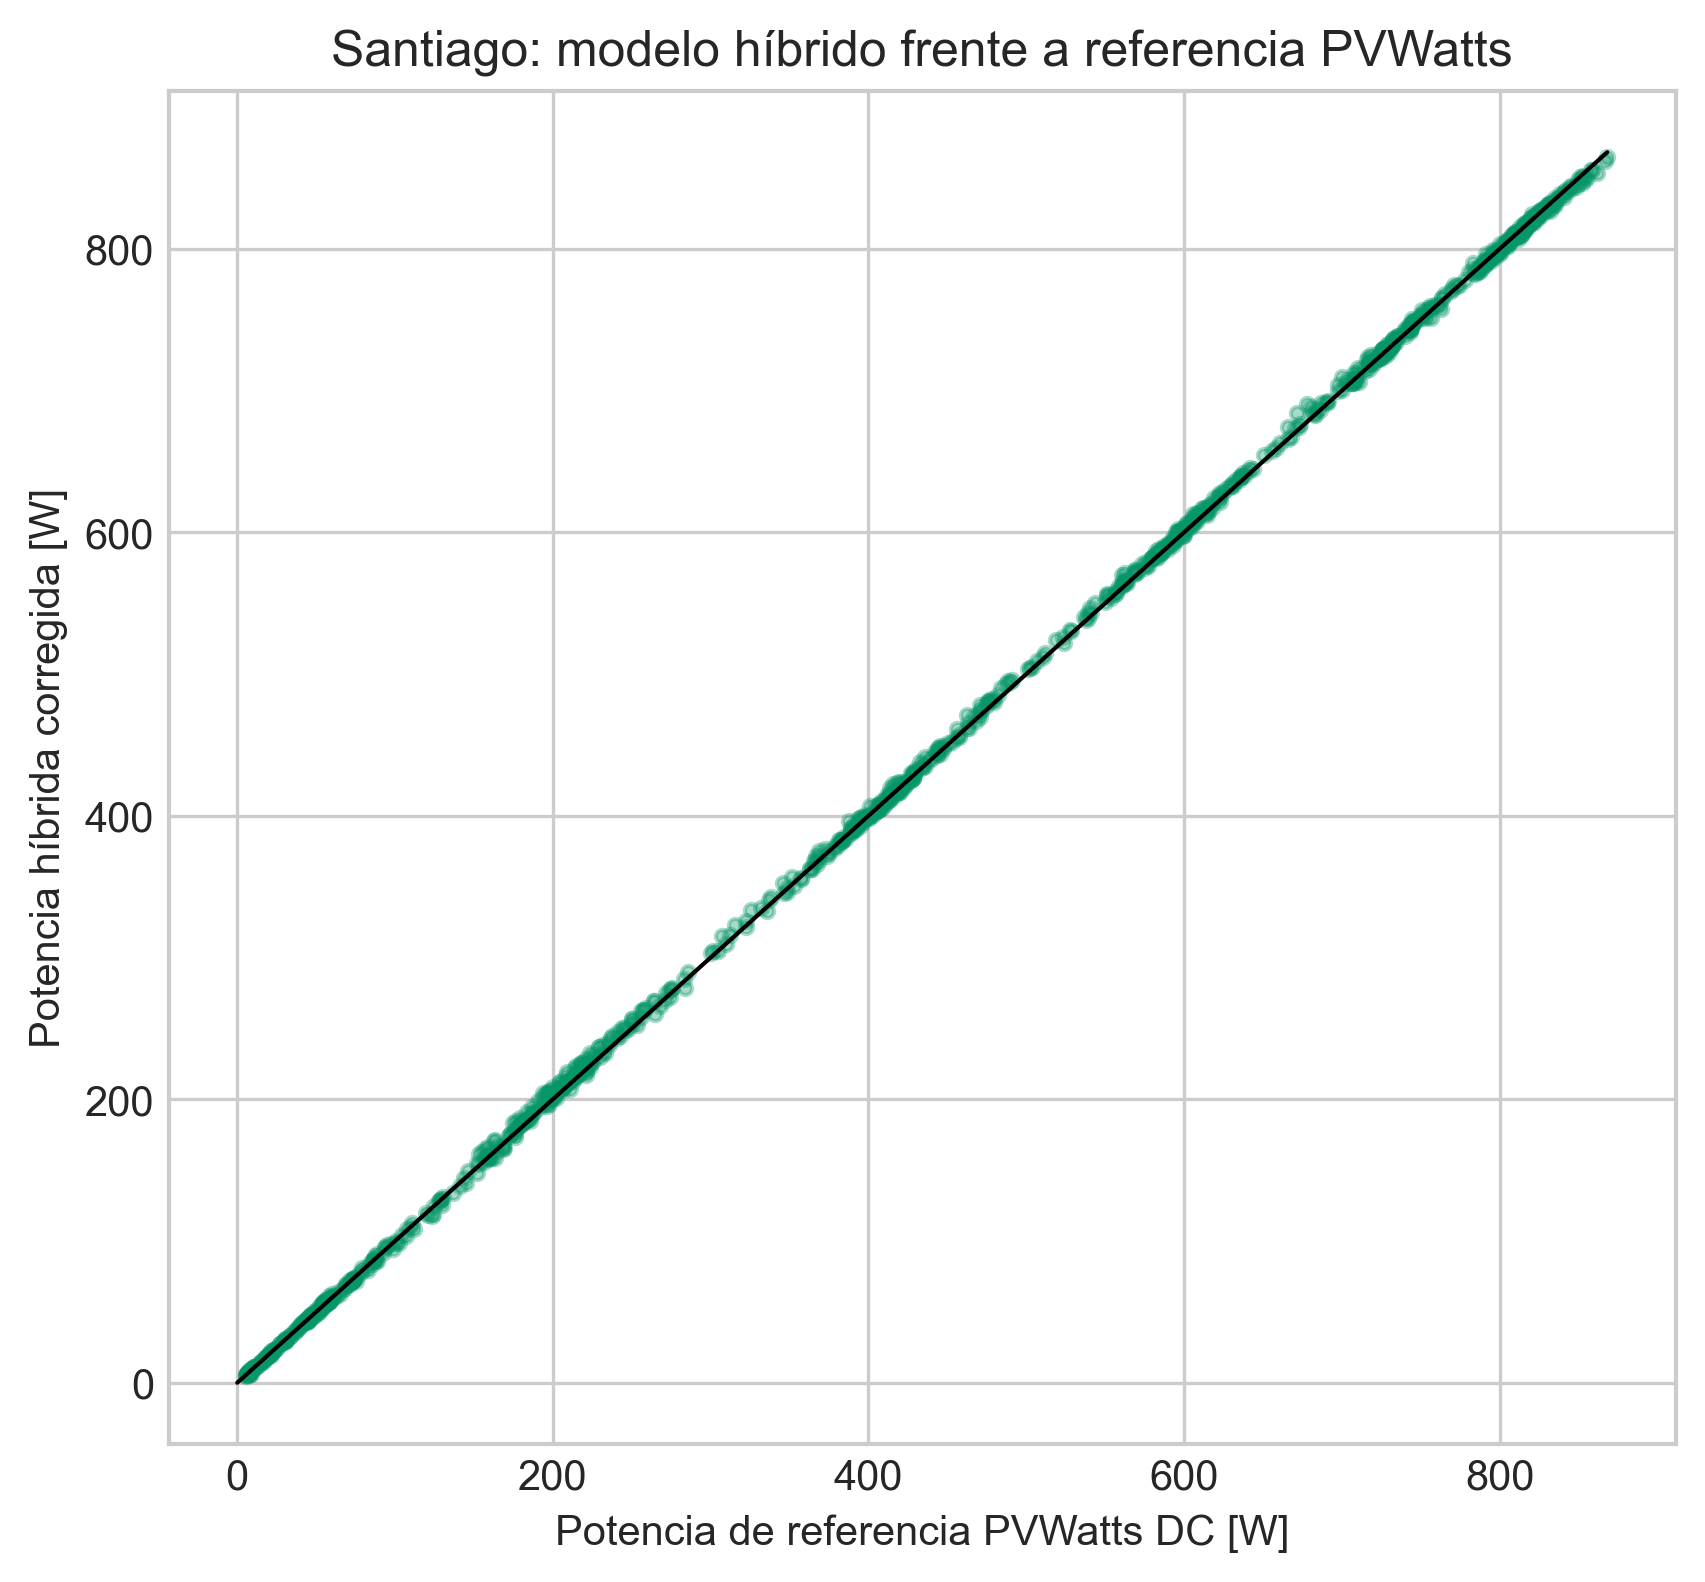
\includegraphics[width=0.72\textwidth]{scatter_phybrid_con_fd_vs_pref_santiago.png}
    \caption{Comparaci\'on entre potencia h\'ibrida corregida y potencia de referencia PVWatts en el conjunto de prueba.}
    \label{fig:phybrid_pref}
\end{figure}

La Figura \ref{fig:phybrid_pref} muestra que la potencia corregida por el modelo h\'ibrido mantiene una alta concordancia con la referencia simulada en el conjunto de prueba. El recorte a cero aplicado por consistencia f\'isica no se activ\'o en este conjunto. Emp\'iricamente, se verific\'o que en todas las fases de modelado (entrenamiento, prueba y validaci\'on cruzada en 5 pliegues) las potencias h\'ibridas corregidas crudas siempre se mantuvieron en niveles positivos, lo que equivale a una frecuencia de activaci\'on del clipping del 0,00\%. Esto evidencia que el modelo residual no requiere truncamientos artificiales invasivos bajo este esquema metodol\'ogico.

La importancia de variables del modelo con fracci\'on difusa se muestra en la Tabla \ref{tab:importancia_xgboost} y en la Figura \ref{fig:importancia_xgboost}. Se reportan las cinco variables de mayor importancia entre las ocho variables de entrada del modelo con \(fd\). La importancia corresponde a la ganancia normalizada utilizada por XGBoost para cuantificar cu\'anto contribuyen las divisiones asociadas a cada variable dentro del ensamble. La fracci\'on difusa aparece como la variable de mayor importancia relativa dentro del modelo entrenado. Esta observaci\'on no debe interpretarse como causalidad f\'isica directa, pero s\'i como evidencia de que \(fd\) aporta informaci\'on predictiva para la correcci\'on residual.

\begin{table}[H]
\centering
\caption{Cinco variables con mayor importancia relativa en el modelo h\'ibrido con fracci\'on difusa.}
\label{tab:importancia_xgboost}
\begin{tabular}{lr}
\toprule
\textbf{Variable} & \textbf{Importancia} \\
\midrule
Fracci\'on difusa & 0,299 \\
Velocidad de viento & 0,239 \\
Irradiancia en el plano del panel & 0,157 \\
Temperatura ambiente & 0,142 \\
Hora, componente seno & 0,062 \\
\bottomrule
\end{tabular}
\end{table}

\begin{figure}[H]
    \centering
    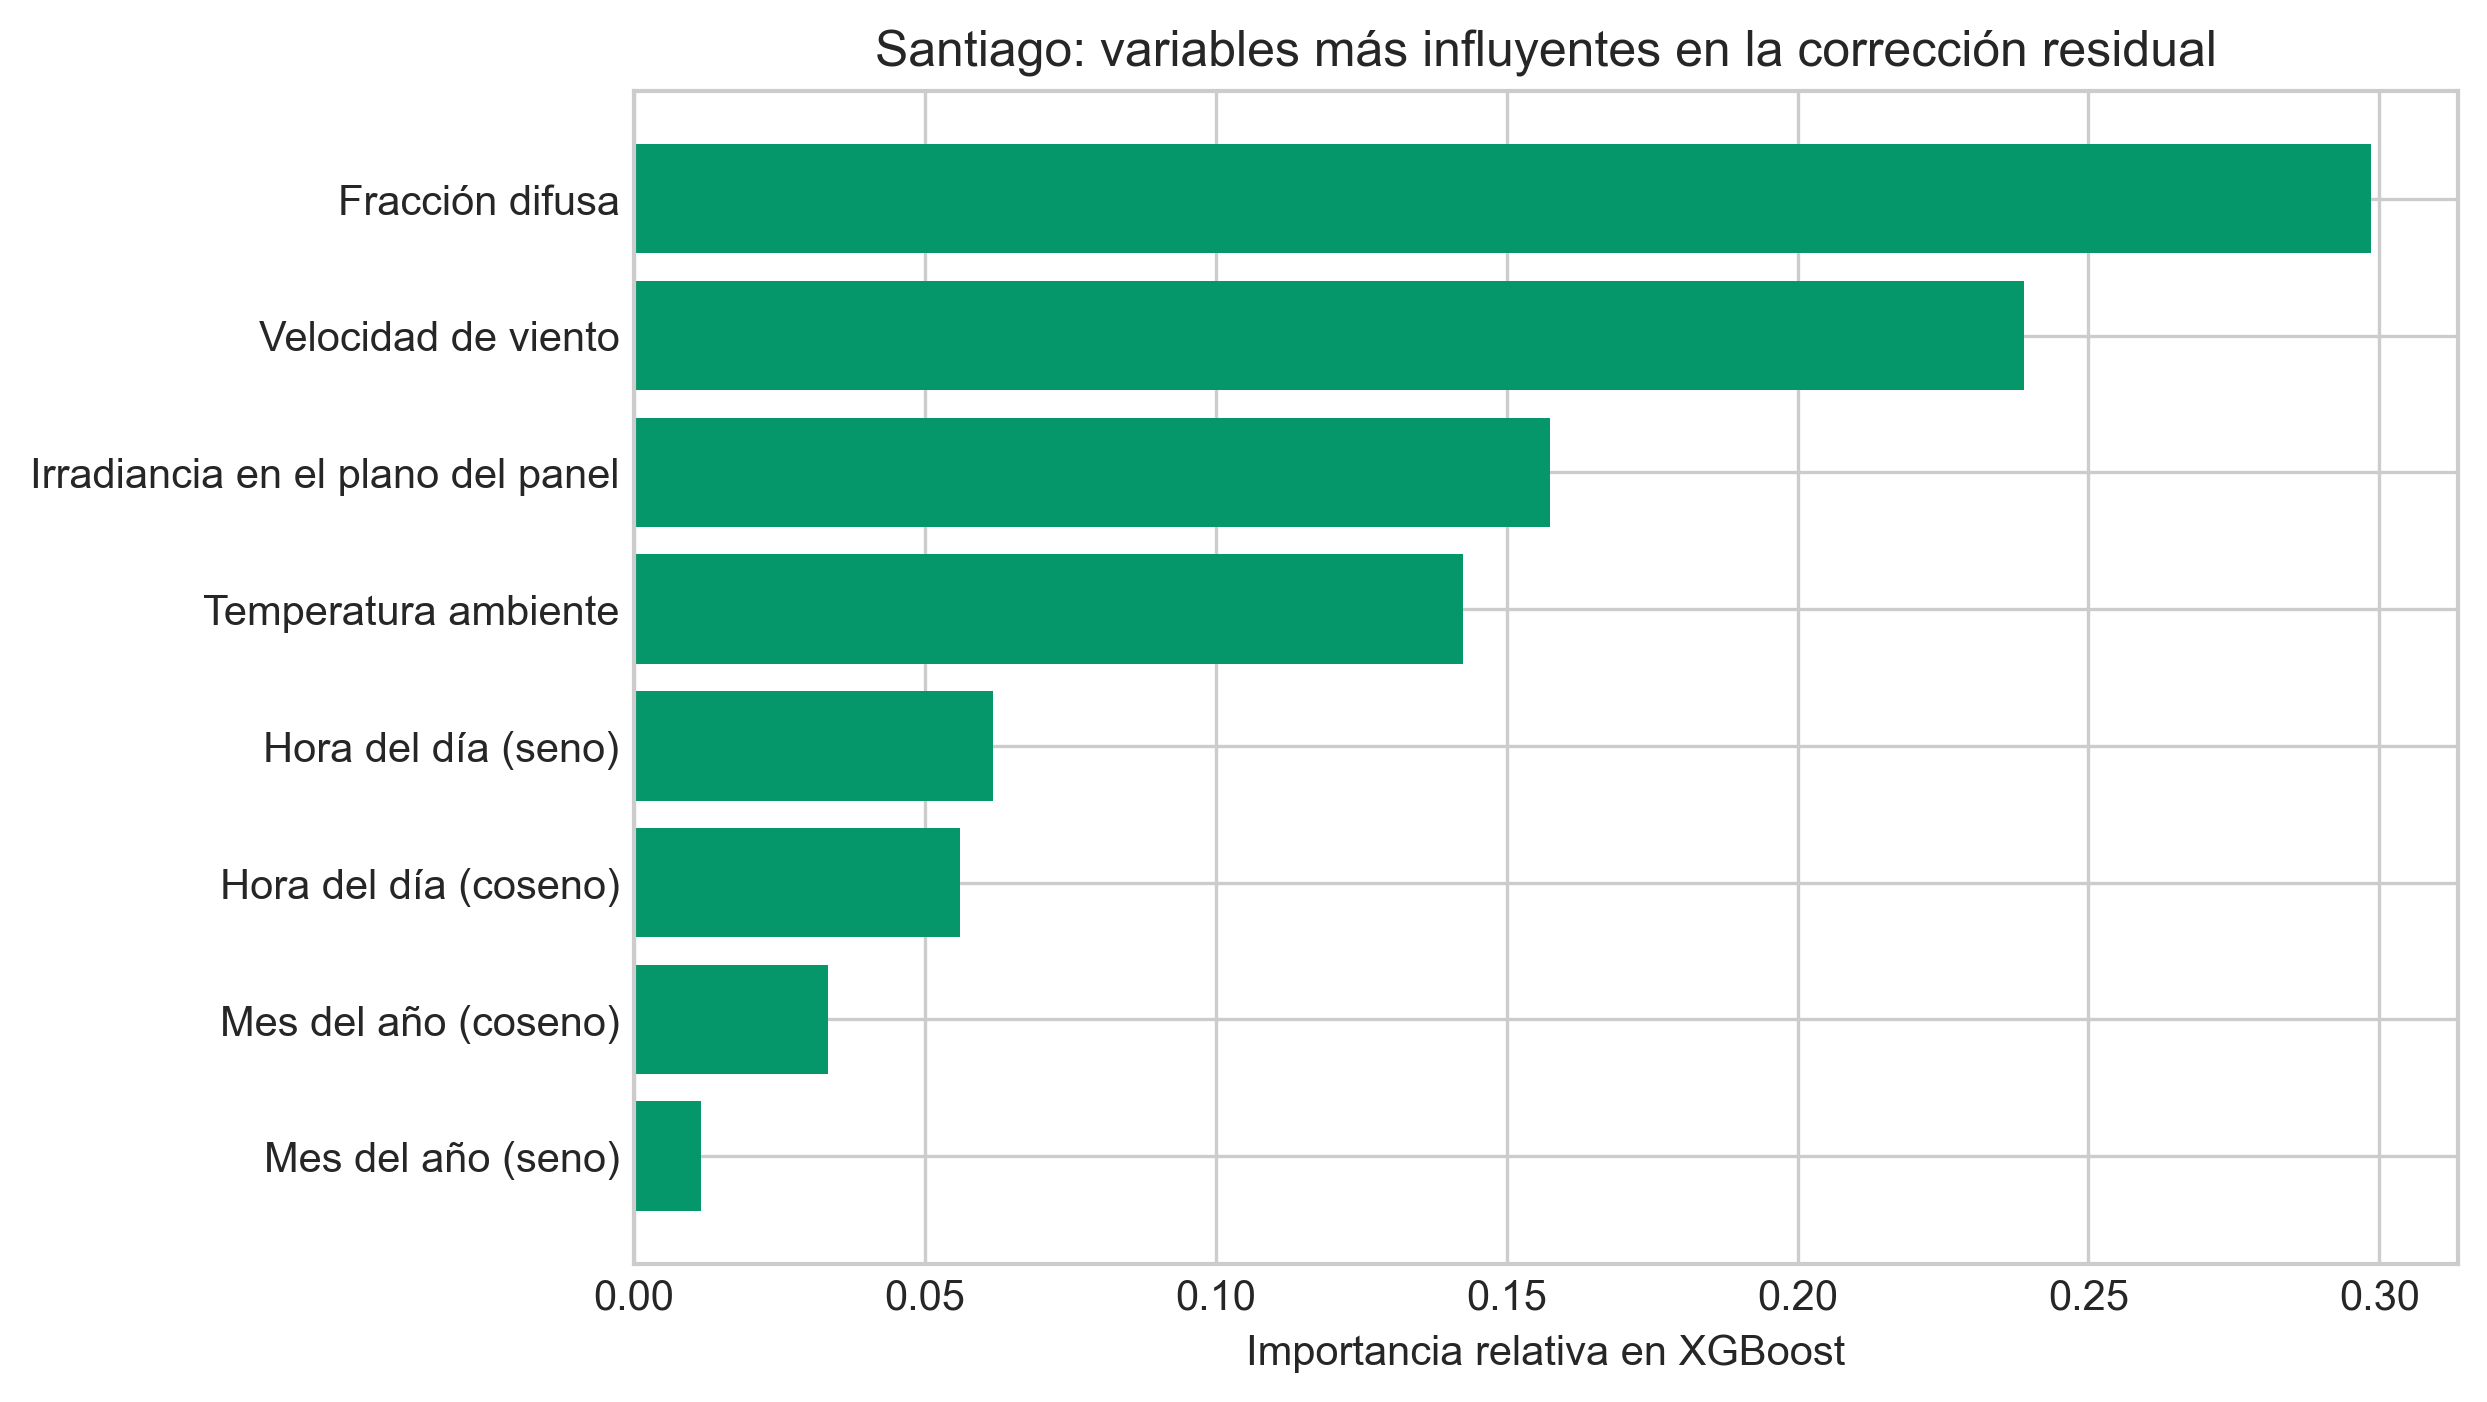
\includegraphics[width=0.76\textwidth]{bar_importancia_xgboost_con_fd_santiago.png}
    \caption{Importancia de variables del modelo h\'ibrido con fracci\'on difusa.}
    \label{fig:importancia_xgboost}
\end{figure}

\subsection{Validaci\'on temporal complementaria}

Adem\'as del conjunto de prueba final, se realiz\'o una validaci\'on temporal con cinco particiones crecientes mediante \texttt{TimeSeriesSplit}. Esta verificaci\'on permite evaluar si la mejora del modelo con fracci\'on difusa se mantiene en distintos bloques temporales. La Tabla \ref{tab:validacion_temporal} reporta el promedio y la desviaci\'on est\'andar muestral de las m\'etricas calculadas sobre las cinco particiones.

\begin{table}[H]
\centering
\caption{Resumen de validaci\'on temporal con cinco particiones, reportando promedio \(\pm\) desviaci\'on est\'andar muestral.}
\label{tab:validacion_temporal}
\resizebox{\textwidth}{!}{%
\begin{tabular}{lrrr}
\toprule
\textbf{Modelo} & \textbf{MAE promedio [W]} & \textbf{RMSE promedio [W]} & \textbf{Error rel. promedio [\%]} \\
\midrule
H\'ibrido sin fracci\'on difusa & \(3,37 \pm 1,32\) & \(4,44 \pm 1,60\) & \(1,38 \pm 0,75\) \\
H\'ibrido con fracci\'on difusa & \(2,52 \pm 0,64\) & \(3,36 \pm 0,85\) & \(1,04 \pm 0,30\) \\
\bottomrule
\end{tabular}%
}
\end{table}

El modelo con fracci\'on difusa obtiene menor MAE promedio que el modelo sin fracci\'on difusa en la validaci\'on temporal. Adem\'as, obtiene menor MAE en las cinco particiones temporales evaluadas y la desviaci\'on est\'andar del MAE disminuye, lo que sugiere un desempe\~no m\'as estable entre particiones temporales. En conjunto, estos resultados respaldan la incorporaci\'on de la fracci\'on difusa dentro del modelo h\'ibrido residual.

% ============================================================
% DISCUSION
% ============================================================

\section{Discusi\'on}

Los resultados muestran que el modelo NOCT, una vez ajustado para considerar p\'erdidas globales equivalentes a las usadas en PVWatts, presenta un buen ajuste general respecto a la potencia simulada de referencia. Esto es esperable, dado que ambos enfoques comparten una dependencia fuerte con la irradiancia sobre el plano del arreglo fotovoltaico. No obstante, el alto \(R^2\) global no implica ausencia de error estructurado.

El an\'alisis por r\'egimen de fracci\'on difusa muestra que el error del modelo NOCT no es uniforme. En baja fracci\'on difusa se observa mayor error absoluto, asociado a condiciones de mayor irradiancia y potencia disponible. En cambio, en alta fracci\'on difusa el error absoluto disminuye, pero el error relativo aumenta. Adem\'as, el signo del bias cambia entre reg\'imenes: bajo baja fracci\'on difusa \(P_{NOCT}\) tiende a subestimar la referencia simulada, mientras que bajo alta fracci\'on difusa tiende a sobreestimarla. Esta transici\'on indica que el residuo contiene estructura asociada al r\'egimen radiativo.

La correlaci\'on entre \(fd\) y las medidas de error respalda esta interpretaci\'on. La correlaci\'on negativa entre \(fd\) y \(\epsilon\) muestra que el residuo cambia sistem\'aticamente con la fracci\'on difusa, mientras que la correlaci\'on positiva entre \(fd\) y el error relativo indica que el error proporcional tiende a aumentar cuando la componente difusa domina. Por tanto, \(fd\) es una variable diagn\'ostica relevante para entender cu\'ando el modelo f\'isico simplificado pierde precisi\'on relativa.

El modelo h\'ibrido residual confirma que el residuo del modelo NOCT no es puramente aleatorio. En el conjunto temporal de prueba, el modelo h\'ibrido sin fracci\'on difusa reduce el MAE desde \SI{13.30}{\watt} hasta \SI{2.70}{\watt}. Esto indica que variables como \(POA\), temperatura, viento, hora y estacionalidad contienen informaci\'on suficiente para corregir parte importante de la discrepancia entre NOCT y PVWatts. Al incorporar la fracci\'on difusa, el MAE disminuye adicionalmente hasta \SI{2.22}{\watt}, y la validaci\'on temporal tambi\'en muestra menor MAE promedio para el modelo que incluye esta variable. Por lo tanto, la fracci\'on difusa aporta informaci\'on incremental respecto al conjunto de variables base considerado.

La importancia de la velocidad de viento tambi\'en entrega una lectura f\'isica de gran relevancia, posicion\'andose como la segunda variable m\'as importante del ensamble (0,239). Esto es coherente con una limitaci\'on evidente del modelo NOCT utilizado: su formulaci\'on estima la temperatura de celda a partir de \(POA\) y temperatura ambiente, pero ignora expl\'icitamente el enfriamiento convectivo por viento. Puesto que el viento captura gran parte de la se\~nal residual, es necesario debatir si el aporte del modelo \textit{con fd} podr\'ia, en menor medida, estar compensando alg\'un efecto secundario del balance t\'ermico en el modelo PVWatts subyacente. En cualquier caso, parte sustancial del residuo modelado por XGBoost claramente responde a diferencias de balance t\'ermico no capturadas inicialmente.

La mejora debe leerse junto con el dise\~no de comparaci\'on. El modelo sin fracci\'on difusa no recibe \(DNI\), \(DHI\) ni \(GHI\), porque esas variables permitir\'ian reconstruir \(fd\) de manera indirecta. De esta forma, la comparaci\'on no favorece artificialmente al modelo base ni al modelo con \(fd\): ambos comparten las mismas variables meteorol\'ogicas y temporales, y solo difieren en la presencia expl\'icita de la fracci\'on difusa. Esta decisi\'on hace que la mejora observada sea una evidencia m\'as directa del aporte incremental de \(fd\).

La elecci\'on de XGBoost tambi\'en debe interpretarse desde el tipo de datos disponible. La base final contiene variables tabulares horarias y un n\'umero de observaciones v\'alidas moderado. En este escenario, un modelo de aprendizaje profundo podr\'ia introducir mayor complejidad, m\'as hiperpar\'ametros y menor interpretabilidad sin garantizar una mejora proporcional. XGBoost ofrece una alternativa m\'as adecuada para esta etapa: modela no linealidades, permite regularizaci\'on, trabaja bien con datos tabulares y entrega una medida diagn\'ostica de importancia de variables. Por ello, el coraz\'on del enfoque no es la profundidad de una red neuronal, sino el acoplamiento entre un modelo f\'isico interpretable y un corrector residual supervisado.

Es crucial precisar el l\'imite de atribuci\'on causal de esta conclusi\'on. La correlaci\'on observada entre la fracci\'on difusa y el residuo del modelo NOCT sugiere una asociaci\'on, pero no implica directamente causalidad f\'isica. El residuo podr\'ia reflejar, parcial o totalmente, otras diferencias estructurales internas entre la simple ecuaci\'on de temperatura de celda y el motor de c\'alculo m\'as robusto integrado en PVWatts. Los resultados no demuestran que \(fd\) sea la \'unica causa f\'isica intr\'inseca del error ni que explique por s\'i sola todas las discrepancias de este modelo simplificado. La potencia de referencia proviene de PVWatts, no de mediciones reales, por lo que el modelo h\'ibrido aprende a corregir NOCT respecto a una referencia simulada. Aun s\'i, dentro de este marco metodol\'ogico, la comparaci\'on controlada entre modelos con y sin \(fd\) entrega evidencia consistente de que la fracci\'on difusa mejora la correcci\'on residual.

% ============================================================
% ALCANCES Y LIMITACIONES
% ============================================================

\section{Alcances y limitaciones}

\begin{enumerate}
    \item La potencia de referencia utilizada corresponde a una simulaci\'on de PVWatts, no a una medici\'on experimental real de un panel fotovoltaico.
    \item La serie horaria descargada corresponde a un a\~no meteorol\'ogico t\'ipico, no a una serie hist\'orica real medida en Santiago.
    \item Para Santiago se utiliz\'o el dataset internacional de PVWatts, ya que la API no encontr\'o datos disponibles bajo \texttt{dataset=nsrdb}.
    \item La fuente clim\'atica efectiva reportada por PVWatts corresponde a Santiago, Chile, con distancia cero respecto de las coordenadas usadas en la consulta. Por tanto, se elimina la inconsistencia espacial entre ubicaci\'on solicitada y fuente clim\'atica efectiva.
    \item La reconstrucci\'on de \(GHI\) se realiz\'o usando la geometr\'ia solar de las coordenadas efectivas de Santiago. Sin embargo, \(DNI\), \(DHI\), \(POA\), temperatura y potencia PVWatts provienen de la simulaci\'on entregada por la plataforma.
    \item El \(POA\) utilizado proviene directamente de la salida horaria de PVWatts. No fue calculado de forma independiente a partir de \(GHI\), \(DHI\), \(DNI\) y geometr\'ia solar.
    \item El modelo NOCT implementado utiliza par\'ametros est\'andar y no fue calibrado con mediciones reales.
    \item El modelo h\'ibrido fue entrenado y evaluado respecto a la misma fuente simulada de referencia. Por tanto, su desempe\~no no debe interpretarse como validaci\'on experimental en terreno.
    \item El modelo h\'ibrido debe interpretarse como un corrector residual de NOCT respecto a PVWatts. No reemplaza una validaci\'on con mediciones reales ni constituye por s\'i solo un sistema de pron\'ostico operacional.
    \item No se entrenaron modelos de aprendizaje profundo. La tesis utiliza aprendizaje autom\'atico supervisado con XGBoost, elegido por su buen comportamiento en datos tabulares, menor complejidad relativa e interpretabilidad diagn\'ostica.
    \item El c\'alculo de \(fd\) excluye horas con \(GHI \leq \SI{10}{\watt\per\square\meter}\), y el error relativo se calcula solo cuando \(P_{ref} > \SI{50}{\watt}\). Estos filtros reducen distorsiones num\'ericas, pero condicionan la interpretaci\'on de las m\'etricas porcentuales.
    \item El estudio considera una ubicaci\'on, una configuraci\'on fotovoltaica fija y un a\~no meteorol\'ogico t\'ipico. La generalizaci\'on a otras zonas clim\'aticas, inclinaciones, tecnolog\'ias de m\'odulo o bases meteorol\'ogicas requiere evaluaciones adicionales.
    \item Las importancias de variables de XGBoost deben interpretarse como indicadores predictivos internos del modelo, no como una demostraci\'on causal de los mecanismos f\'isicos involucrados.
\end{enumerate}

% ============================================================
% CONCLUSIONES PARCIALES
% ============================================================

\section{Conclusiones}

El desarrollo de este proyecto permiti\'o dar respuesta a la pregunta de investigaci\'on mediante una secuencia alineada con los cinco objetivos espec\'ificos propuestos. A partir de los resultados, se concluye lo siguiente:

\begin{enumerate}
    \item \textbf{Construcci\'on de base y clasificaci\'on (Obj. 1):} Se consolid\'o con \'exito una base horaria simulada para Santiago, obteniendo observaciones balanceadas (1349 en baja fracci\'on difusa, 1126 en r\'egimen mixto y 1740 en alta fracci\'on difusa). Esto confirma que la definici\'on metodol\'ogica de \(fd = DHI/GHI\) fue operable y discriminante sobre los datos clim\'aticos utilizados.
    \item \textbf{Implementaci\'on del modelo f\'isico (Obj. 2):} El modelo f\'isico NOCT reprodujo adecuadamente la tendencia principal de la generaci\'on (\(R^2 = 0{,}9968\)). Sin embargo, su precisi\'on fluctu\'o, mostrando errores absolutos dominantes en alta irradiancia y sesgos relativos dependientes de la fracci\'on difusa.
    \item \textbf{Diagn\'ostico del residuo (Obj. 3):} El residuo del modelo NOCT demostr\'o emp\'iricamente no ser aleatorio. Se comprob\'o una asociaci\'on sistem\'atica (\(p < 0{,}01\)) con la fracci\'on difusa, revelando que en alta \(fd\) el modelo f\'isico tiende a sobreestimar la producci\'on relativa, lo que degrada la estimaci\'on porcentual bajo irradiancia dispersa.
    \item \textbf{Correcci\'on residual con aprendizaje autom\'atico (Obj. 4):} El entrenamiento de modelos h\'ibridos sobre el residuo f\'isico logr\'o reducir dram\'aticamente el error del modelo base. La aproximaci\'on demostr\'o que variables como temperatura, radiaci\'on incidente y velocidad de viento (esta \'ultima fundamental en el balance t\'ermico no capturado por NOCT) albergan se\~nales suficientes para minimizar las discrepancias (reduciendo el MAE de prueba de \SI{13.30}{\watt} a \SI{2.70}{\watt}).
    \item \textbf{Aporte incremental de la fracci\'on difusa (Obj. 5):} Al comparar el modelo h\'ibrido sin \(fd\) frente al modelo con \(fd\), el MAE de prueba se redujo adicionalmente un 17,69\% (hasta \SI{2.22}{\watt}), sin activaci\'on artificial de recortes por truncamiento f\'isico (0\% clipping). Esto confirma emp\'iricamente la hip\'otesis: incorporar la fracci\'on difusa provee informaci\'on estructural predictiva novedosa, validando as\'i su valor y aporte general.
\end{enumerate}

Por consiguiente, el objetivo general de la investigaci\'on se declara cumplido. La fracci\'on difusa prob\'o ser tanto un diagn\'ostico revelador de las debilidades t\'ermico--radiativas de modelos f\'isicos simples, como un atributo clave para enriquecer modelos de regresi\'on h\'ibrida orientados a la estimaci\'on fotovoltaica. Naturalmente, la principal limitaci\'on a abordar a futuro es el car\'acter simulado de la referencia (PVWatts), abriendo v\'ias para un futuro escalamiento y validaci\'on experimental.

% ============================================================
% TRABAJO SIGUIENTE
% ============================================================

\section{Trabajo futuro}

Como extensi\'on natural de este trabajo, se propone validar el flujo metodol\'ogico con mediciones reales de potencia fotovoltaica, irradiancia y meteorolog\'ia local. Esta validaci\'on permitir\'ia determinar si la mejora observada frente a PVWatts se mantiene respecto a un sistema f\'isico instrumentado.

Tambi\'en se recomienda ampliar el an\'alisis a m\'as ubicaciones, distintos reg\'imenes clim\'aticos, diferentes inclinaciones y tecnolog\'ias de m\'odulo. Esto permitir\'ia evaluar la generalidad del aporte de \(fd\) y distinguir si su relevancia depende de condiciones atmosf\'ericas o geom\'etricas particulares.

Otra l\'inea de trabajo consiste en calcular el \(POA\) de forma independiente a partir de \(GHI\), \(DNI\), \(DHI\), geometr\'ia solar y modelos de transposici\'on, en lugar de utilizar directamente el \(POA\) entregado por PVWatts. Esto permitir\'ia separar mejor las fuentes de error asociadas a geometr\'ia, irradiancia y temperatura.

Finalmente, se podr\'ian explorar estrategias de optimizaci\'on de hiperpar\'ametros con validaci\'on temporal anidada, modelos con incertidumbre predictiva y m\'etodos de interpretabilidad como SHAP. En una etapa posterior, tambi\'en podr\'ian evaluarse modelos de aprendizaje profundo si se dispone de bases m\'as extensas, m\'ultiples ubicaciones o secuencias meteorol\'ogicas de mayor complejidad. Estas extensiones ayudar\'ian a robustecer la interpretaci\'on del modelo h\'ibrido y su posible uso en aplicaciones de estimaci\'on o predicci\'on fotovoltaica.

% ============================================================
% REFERENCIAS
% ============================================================

\newpage
\begin{thebibliography}{9}

\bibitem{ramadhan2021}
Ramadhan, R.~W. y Naseem, A. (2021).
\textit{Recent Trends in Photovoltaic Power Forecasting}.
Energies, 14(20), 6610.

\bibitem{erbs1982}
Erbs, D.~G., Klein, S.~A. y Duffie, J.~A. (1982).
\textit{Estimation of the diffuse radiation fraction for hourly, daily and monthly-average global radiation}.
Solar Energy, 28(4), 293--302.

\bibitem{pvwatts2026}
NREL (2026).
\textit{PVWatts Calculator}.
National Renewable Energy Laboratory. \url{https://pvwatts.nrel.gov/}

\bibitem{xgboost2016}
Chen, T. y Guestrin, C. (2016).
\textit{XGBoost: A Scalable Tree Boosting System}.
Actas de la 22.a Conferencia Internacional ACM SIGKDD sobre Descubrimiento de Conocimiento y Miner\'ia de Datos.

\bibitem{mayer2022}
Mayer, M.~J. y Gr\'of, G. (2022).
\textit{Benefits of physical and machine learning hybridization for photovoltaic power forecasting}.
Renewable and Sustainable Energy Reviews, 168, 112772.

\bibitem{santos2024}
Santos, L.~O., et al. (2024).
\textit{Photovoltaic power estimation and forecast models integrating physics and machine learning: A review on hybrid techniques}.
Solar Energy, 270, 112377.

\end{thebibliography}

\newpage
\appendix
\section{Anexo: Glosario de Conceptos}

\begin{description}
    \item[\textit{Residual learning} (aprendizaje residual):] Enfoque de modelado donde un algoritmo de aprendizaje autom\'atico no predice directamente el valor objetivo final, sino la discrepancia (o residuo) respecto a una aproximaci\'on previa (como un modelo f\'isico). Esto facilita que el algoritmo se concentre solo en capturar los fen\'omenos complejos no modelados inicialmente.
    \item[\texttt{pvlib}:] Biblioteca de c\'odigo abierto en lenguaje Python especializada en la simulaci\'on de rendimiento de sistemas de energ\'ia solar fotovoltaica. Provee funciones estandarizadas para c\'alculos astron\'omicos, irradiancia, t\'ermicos y el\'ectricos.
    \item[\'Angulo cenital solar (\(\theta_z\)):] \'Angulo que se forma entre la direcci\'on del sol y el cenit (la vertical exacta del lugar). Se calcula algor\'itmicamente en funci\'on de la latitud, longitud, altitud y fecha, y determina qu\'e proporci\'on de la radiaci\'on directa normal (\(DNI\)) incide sobre un plano horizontal.

\end{description}

\end{document}
